\subsection{\texorpdfstring{Computation of the modules \(\operatorname{Tor}^{\mathbf{A}}(\mathbf{P},\mathbf{M})\) and \(\operatorname{Ext}_{\mathbf{A}}(\mathbf{M},\mathbf{N})\)}{Computation of the modules \textbackslash operatorname\{Tor\}\^{}\{\textbackslash mathbf\{A\}\}(\textbackslash mathbf\{P\},\textbackslash mathbf\{M\}) and \textbackslash operatorname\{Ext\}\_\{\textbackslash mathbf\{A\}\}(\textbackslash mathbf\{M\},\textbackslash mathbf\{N\})}}

Let M, N be left A-modules, P a right A-module. Let moreover \(a: R \rightarrow M\) be a left resolution of M, \(b: S \rightarrow P\) a left resolution of P, and \(c: N \rightarrow E\) a right resolution of N.

By X, p.~49, prop. 3 and 3 bis, there exist morphisms of complexes \(\alpha: L(M) \to R\) , \(\beta: L(P) \to S\) , \(\gamma: E \to I(N)\) such that \(a \circ \alpha = p_{M}\) , \(b \circ \beta = p_{P}\) , \(\gamma \circ c = e_{N}\) ; and the homotopy classes of \(\alpha\) , \(\beta\) , \(\gamma\) depend only on the given resolutions. By X, p.~64, prop. 3 and X, p.~84, prop. 3, the homotopy classes of the morphisms

\[
\beta \otimes \alpha : L (P) \otimes_ {A} L (M) \rightarrow S \otimes_ {A} R,
\]

\[
\operatorname{Homgr} _ {\mathbf {A}} (\alpha , \gamma): \operatorname{Homgr} _ {\mathbf {A}} (\mathrm{R}, \mathrm{E}) \rightarrow \operatorname{Homgr} _ {\mathbf {A}} (\mathrm{L} (\mathrm{M}), \mathrm{I} (\mathrm{N}))
\]

depend only on the given resolutions, whence, by passing to homology, graded k-homomorphisms of degree 0

\[
\psi (\mathrm{S}, \mathrm{R}): \operatorname{Tor} ^ {\mathrm{A}} (\mathrm{P}, \mathrm{M}) \rightarrow \mathrm{H} (\mathrm{S} \otimes_ {\mathrm{A}} \mathrm{R}),
\]

\[
\varphi (\mathrm{R}, \mathrm{E}): \mathrm{H} \left(\operatorname{Homgr} _ {\mathrm{A}} (\mathrm{R}, \mathrm{E})\right)\rightarrow \operatorname{Ext} _ {\mathrm{A}} (\mathrm{M}, \mathrm{N}),
\]

independent of the choices of α, β, γ.

For example, taking for \(a\) , \(b\) , \(c\) the identity maps of M, P, N respectively, one obtains the homomorphisms \(\psi(\mathbf{P}, \mathbf{M}) : \operatorname{Tor}^{\mathbf{A}}(\mathbf{P}, \mathbf{M}) \to \mathbf{P} \otimes_{\mathbf{A}} \mathbf{M}\) and \(\varphi(\mathbf{M}, \mathbf{N}) : \operatorname{Hom}_{\mathbf{A}}(\mathbf{M}, \mathbf{N}) \to \operatorname{Ext}_{\mathbf{A}}(\mathbf{M}, \mathbf{N})\) introduced in X, p.~68, remark 2) and X, p.~87, remark 2).

THEOREM 1. --- a) If one of the resolutions R or S is flat, then \(\psi(S, R)\) is an isomorphism of \(k\) -graded modules.

\begin{enumerate}
\def\labelenumi{\alph{enumi})}
\setcounter{enumi}{1}
\item
  If R is projective or if E is injective, \(\varphi(\mathbf{R},\mathbf{E})\) is an isomorphism of \(k\) -graded modules.
\item
  Suppose for example R is flat, and choose \(\alpha\) and \(\beta\) as above. The homomorphism \(\beta \otimes \alpha\) is the composite of the morphisms
\end{enumerate}

\[
\mathrm{L} (\mathrm{P}) \otimes_ {\mathrm{A}} \mathrm{L} (\mathrm{M}) \xrightarrow {l _ {\mathrm{L} (\mathrm{P})} \otimes \alpha} \mathrm{L} (\mathrm{P}) \otimes_ {\mathrm{A}} \mathrm{R} \xrightarrow {\beta \otimes 1 _ {\mathrm{R}}} \mathrm{S} \otimes_ {\mathrm{A}} \mathrm{R}.
\]

Since L(P) (resp. R) is flat and \(\alpha\) (resp. \(\beta\) ) is a homology isomorphism, \(1_{L(P)} \otimes \alpha\) (resp. \(\beta \otimes 1_R\) ) is one, by prop. 4 of X, p.~67. Hence \(\beta \otimes \alpha\) is a homology isomorphism and \(\psi(S, R) = H(\beta \otimes \alpha)\) is bijective.

\begin{enumerate}
\def\labelenumi{\alph{enumi})}
\setcounter{enumi}{1}
\tightlist
\item
  One argues similarly, using prop. 4 of X, p.~86.
\end{enumerate}

COROLLARY. --- If R is a flat resolution of M, the homomorphism

\[
\psi (\mathrm{P}, \mathrm{R}): \operatorname{Tor} ^ {\mathbf {A}} (\mathrm{P}, \mathrm{M}) \rightarrow \mathrm{H} (\mathrm{P} \otimes_ {\mathbf {A}} \mathrm{R})
\]

is bijective. If R is a projective resolution of M, the homomorphism

\[
\varphi (\mathrm{R}, \mathrm{N}): \mathrm{H} \left(\operatorname{Homgr} _ {\mathrm{A}} (\mathrm{R}, \mathrm{N})\right)\rightarrow \operatorname{Ext} _ {\mathrm{A}} (\mathrm{M}, \mathrm{N})
\]

is bijective. If E is an injective resolution of N, the homomorphism

\[
\varphi (\mathbf {M}, \mathbf {E}): \mathrm{H} \left(\operatorname{Homgr} _ {\mathbf {A}} (\mathbf {M}, \mathbf {E})\right)\rightarrow \operatorname{Ext} _ {\mathbf {A}} (\mathbf {M}, \mathbf {N})
\]

is bijective.

Remark. --- The diagram of k-modules

\[
\begin{array}{c} \operatorname{Tor} ^ {\mathbf {A}} (\mathrm{P}, \mathrm{M}) \xrightarrow {\psi (\mathrm{S} , \mathrm{R})} \mathrm{H} (\mathrm{S} \otimes_ {\mathbf {A}} \mathrm{R}) \\ \sigma_ {\mathrm{P}, \mathrm{M}} \Biggl \downarrow \\ \operatorname{Tor} ^ {\mathbf {A} ^ {\circ}} (\mathrm{M} ^ {\circ}, \mathrm{P} ^ {\circ}) \xrightarrow {\psi (\mathrm{R} ^ {\circ} , \mathrm{S} ^ {\circ})} \mathrm{H} (\mathrm{R} ^ {\circ} \otimes_ {\mathbf {A} ^ {\circ}} \mathrm{S} ^ {\circ}), \end{array}
\]

where \(\sigma_{\mathrm{P,M}}\) and \(\sigma(\mathrm{S},\mathrm{R})\) are the commutation isomorphisms (X, p.~71 and 63), is commutative: it is indeed deduced, by passing to homology, from the commutative diagram of complexes

\[
\begin{array}{c c} \mathrm{L} (\mathrm{P}) \otimes_ {\mathrm{A}} \mathrm{L} (\mathrm{M}) & \xrightarrow {\beta \otimes \alpha} \mathrm{S} \otimes_ {\mathrm{A}} \mathrm{R} \\ \sigma (\mathrm{L} (\mathrm{P}), \mathrm{L} (\mathrm{M})) \Big \downarrow & \Big \downarrow \sigma (\mathrm{S}, \mathrm{R}) \\ \mathrm{L} (\mathrm{M} ^ {\circ}) \otimes_ {\mathrm{A} ^ {\circ}} \mathrm{L} (\mathrm{P} ^ {\circ}) & \xrightarrow {\alpha \otimes \beta} \mathrm{R} ^ {\circ} \otimes_ {\mathrm{A} ^ {\circ}} \mathrm{S} ^ {\circ} \end{array}
\]

(“the morphisms \(\psi\) are compatible with the commutation isomorphisms”).

Similarly, let \(a_{1}: \mathbb{R}_{1} \to \mathbb{M}\) , \(b_{1}: \mathbb{S}_{1} \to \mathbb{P}\) , \(c_{1}: \mathbb{N} \to \mathbb{E}_{1}\) be morphisms of complexes, where \(\mathbb{R}_{1}\) and \(\mathbb{S}_{1}\) are projective and zero on the right, and \(\mathbb{E}_{1}\) injective and zero on the left. By X, p.~49, prop. 3 and 3 bis, there exist morphisms of complexes

\[
\alpha_ {1}: \mathrm{R} _ {1} \rightarrow \mathrm{L} (\mathrm{M}), \quad \beta_ {1}: \mathrm{S} _ {1} \rightarrow \mathrm{L} (\mathrm{P}), \quad \gamma_ {1}: \mathrm{I} (\mathrm{N}) \rightarrow \mathrm{E} _ {1}
\]

such that \(p_{\mathrm{M}} \circ \alpha_{1} = a_{1}, p_{\mathrm{P}} \circ \beta_{1} = b_{1}, \gamma_{1} \circ e_{\mathrm{N}} = c_{1}\) , whence morphisms of complexes

\[
\beta_ {1} \otimes \alpha_ {1}: S _ {1} \otimes_ {A} R _ {1} \rightarrow L (P) \otimes_ {A} L (M),
\]

\[
\operatorname{Homgr} _ {\mathbf {A}} \left(\alpha_ {1}, \gamma_ {1}\right): \operatorname{Homgr} _ {\mathbf {A}} \left(\mathrm{L} (\mathrm{M}), \mathrm{I} (\mathrm{N})\right)\rightarrow \operatorname{Homgr} _ {\mathbf {A}} \left(\mathrm{R} _ {1}, \mathrm{E} _ {1}\right),
\]

and, by passing to homology, graded k-linear maps of degree 0:

\[
\begin{array}{l} \psi^ {\prime} (\mathbf {S} _ {1}, \mathbf {R} _ {1}): \mathrm{H} (\mathbf {S} _ {1} \otimes_ {\mathbf {A}} \mathbf {R} _ {1}) \to \operatorname{Tor} ^ {\mathbf {A}} (\mathbf {P}, \mathbf {M}) \\ \varphi^ {\prime} (\mathbf {R} _ {1}, \mathbf {E} _ {1}): \operatorname{Ext} _ {\mathbf {A}} (\mathbf {M}, \mathbf {N}) \to \mathrm{H} (\operatorname{Homgr} _ {\mathbf {A}} (\mathbf {R} _ {1}, \mathbf {E} _ {1})) \end{array}
\]

which one verifies as above are independent of the choice of \(\alpha_{1}\) , \(\beta_{1}\) , \(\gamma_{1}\) .

PROPOSITION 1. --- If \(a_{1}\) , \(b_{1}\) , \(c_{1}\) are homology isomorphisms, \(\psi^{\prime}(\mathbf{S}_{1},\mathbf{R}_{1})\) and \(\varphi^{\prime}(\mathbf{R}_{1},\mathbf{E}_{1})\) are the inverse bijections of the bijections \(\psi(\mathbf{S}_{1},\mathbf{R}_{1})\) and \(\varphi(\mathbf{R}_{1},\mathbf{E}_{1})\) respectively. Indeed, \(f = (\beta \otimes \alpha) \circ (\beta_{1} \otimes \alpha_{1})\) is a morphism of the complex \(\mathbf{S}_{1} \otimes_{\mathbf{A}} \mathbf{R}_{1}\) into itself, and one has \((b_{1} \circ \alpha_{1}) \circ f = f\) . By X, p.~49, prop. 3 and 3 bis, \(f\) is a homotopy equivalence, hence H(f) = 1 and

\[
\psi \left(\mathrm{S} _ {1}, \mathrm{R} _ {1}\right) \circ \psi^ {\prime} \left(\mathrm{S} _ {1}, \mathrm{R} _ {1}\right) = \mathrm{H} (\beta \otimes \alpha) \circ \mathrm{H} \left(\beta_ {1} \otimes \alpha_ {1}\right) = \mathrm{H} (f) = 1;
\]

likewise \(\psi'(S_1, R_1) \circ \psi(S_1, R_1) = 1\) . One argues analogously for the maps \(\varphi\) and \(\varphi'\) .

Examples. --- 1) Let \(a\) be an element of A such that the map \(\varphi : x \mapsto xa\) from A into itself be injective ( \(a\) is not a right zero divisor). Using the resolution

\[
0 \rightarrow \mathrm{A} _ {s} \xrightarrow {\varphi} \mathrm{A} _ {s} \rightarrow \mathrm{A} / \mathrm{A} a \rightarrow 0
\]

we see that for every right A-module M, we have

\[
\operatorname{Tor} _ {i} ^ {\mathbf {A}} (\mathbf {M}, \mathbf {A} / \mathbf {A} a) = 0 \quad \text { for } \quad i > 1
\]

and that the \(k\) -module \(\operatorname{Tor}_1^{\mathbf{A}}(\mathbf{M}, \mathbf{A} / \mathbf{A}a)\) is isomorphic to \(\operatorname{Ker}(a_{\mathbf{M}})\) .

Similarly, for every left A-module M, we have

\[
\operatorname{Ext} _ {\mathbf {A}} ^ {i} (\mathbf {A} / \mathbf {A} a, \mathbf {M}) = 0 \quad \text { for } \quad i > 1
\]

and the \(k\) -module \(\operatorname{Ext}_{\mathbf{A}}^{1}(\mathbf{A}/\mathbf{A}a, \mathbf{M})\) is isomorphic to \(\mathbf{M}/a\mathbf{M}\) .

\begin{enumerate}
\def\labelenumi{\arabic{enumi})}
\setcounter{enumi}{1}
\tightlist
\item
  Suppose A is an integral domain; let K be the field of fractions of A and M an A-module. Using the flat resolution
\end{enumerate}

\[
0 \rightarrow \mathrm{A} \rightarrow \mathrm{K} \rightarrow \mathrm{K} / \mathrm{A} \rightarrow 0
\]

(X, p.~9, example 5), we see that \(\operatorname{Tor}_{i}^{\mathbf{A}}(\mathbf{K}/\mathbf{A}, \mathbf{M}) = 0\) for \(i > 1\) ; moreover, taking into account II, p.~116, prop. 26, (ii), the A-module \(\operatorname{Tor}_{1}^{\mathbf{A}}(\mathbf{K}/\mathbf{A}, \mathbf{M})\) is isomorphic to the torsion submodule of M.

\begin{enumerate}
\def\labelenumi{\arabic{enumi})}
\setcounter{enumi}{2}
\tightlist
\item
  Suppose that A is a Noetherian local ring, denote its maximal ideal by m, and set \(\kappa = \mathbf{A} / \mathfrak{m}\) Let M be a finitely generated A-module and P a minimal projective resolution of M (X, p.~54). For every \(n \geqslant 0\) , the \(\kappa\) vector spaces \(\operatorname{Tor}_n^{\mathbf{A}}(\kappa, \mathbf{M})\) and \(\operatorname{Ext}_{\mathbf{A}}^{n}(\mathbf{M}, \kappa)\) are finite-dimensional, of dimension equal to the rank of the free A-module \(\mathbf{P}_n\) ; indeed, the complexes \(\kappa \otimes_{\mathbf{A}} \mathbf{P}\) and \(\operatorname{Homgr}_{\mathbf{A}}(\mathbf{P}, \kappa)\) have zero differential.
\end{enumerate}

\subsection{\texorpdfstring{Computation of the mappings \(\operatorname{Tor}^{\mathbf{A}}(g, f)\) and \(\operatorname{Ext}_{\mathbf{A}}(f, h)\)}{Computation of the mappings \textbackslash operatorname\{Tor\}\^{}\{\textbackslash mathbf\{A\}\}(g, f) and \textbackslash operatorname\{Ext\}\_\{\textbackslash mathbf\{A\}\}(f, h)}}

Let \(f: \mathbf{M} \to \mathbf{M}'\) , \(h: \mathbf{N}' \to \mathbf{N}\) be homomorphisms of left A-modules, \(g: \mathbf{P} \to \mathbf{P}'\) a homomorphism of right A-modules, \(a: \mathbf{R} \to \mathbf{M}\) , \(a': \mathbf{R}' \to \mathbf{M}'\) , \(b: \mathbf{S} \to \mathbf{P}\) , \(b': \mathbf{S}' \to \mathbf{P}'\) left resolutions of M, M', P, P', respectively, \(c: \mathbf{N} \to \mathbf{E}\) , \(c': \mathbf{N}' \to \mathbf{E}'\) right resolutions of N and N', \(\tilde{f}: \mathbf{R} \to \mathbf{R}'\) , \(\tilde{g}: \mathbf{S} \to \mathbf{S}'\) , \(\tilde{h}: \mathbf{E}' \to \mathbf{E}\) morphisms of complexes such that

\[
a ^ {\prime} \circ \tilde {f} = f \circ a, b ^ {\prime} \circ \tilde {g} = g \circ b, \tilde {h} \circ c ^ {\prime} = c \circ h.
\]

PROPOSITION 2. --- The following two diagrams are commutative:

\[
\begin{array}{c} \operatorname{Tor} ^ {\mathbf {A}} (\mathrm{P}, \mathrm{M}) \xrightarrow {\psi (\mathrm{S} , \mathrm{R})} \mathrm{H} (\mathrm{S} \otimes_ {\mathbf {A}} \mathrm{R}) \\ \operatorname{Tor} ^ {\mathbf {A}} (g, f) \Big \downarrow \qquad \qquad \qquad \qquad \qquad \qquad \qquad \qquad \qquad \qquad \qquad \qquad \qquad \qquad \qquad \qquad \qquad \qquad \qquad \qquad \qquad \qquad \qquad \qquad \qquad \qquad \qquad \qquad \qquad \qquad \qquad \qquad \qquad \qquad \\ \operatorname{Tor} ^ {\mathbf {A}} (\mathrm{P} ^ {\prime}, \mathrm{M} ^ {\prime}) \xrightarrow {\psi (\mathrm{S} ^ {\prime} , \mathrm{R} ^ {\prime})} \mathrm{H} (\mathrm{S} ^ {\prime} \otimes_ {\mathbf {A}} \mathrm{R} ^ {\prime})  , \end{array}
\]

\[
\begin{array}{c} \mathrm{H} (\operatorname{Homgr} _ {\mathbf {A}} (\mathrm{R} ^ {\prime}, \mathrm{E} ^ {\prime})) \xrightarrow {\varphi (\mathrm{R} ^ {\prime} , \mathrm{E} ^ {\prime})} \operatorname{Ext} _ {\mathbf {A}} (\mathrm{M} ^ {\prime}, \mathrm{N} ^ {\prime}) \\ \mathrm{H} (\operatorname{Homgr} _ {\mathbf {A}} (\tilde {f}, \tilde {h})) \Biggl \downarrow \\ \mathrm{H} (\operatorname{Homgr} _ {\mathbf {A}} (\mathrm{R}, \mathrm{E})) \xrightarrow {\varphi (\mathrm{R} , \mathrm{E})} \operatorname{Ext} _ {\mathbf {A}} (\mathrm{M}, \mathrm{N}). \end{array}
\]

Let \(\alpha: L(M) \to R\) , \(\alpha': L(M') \to R'\) , \(\gamma: L(P) \to S\) , \(\gamma': L(P') \to S'\) morphisms of complexes such that

\[
a \circ \alpha = p _ {\mathrm{M}}, a ^ {\prime} \circ \alpha^ {\prime} = p _ {\mathrm {M^ {\prime}}}, b \circ \gamma = p _ {\mathrm{P}}, b ^ {\prime} \circ \gamma^ {\prime} = p _ {\mathrm {P^ {\prime}}}.
\]

By definition, \(\mathrm{H}(\tilde{g}\otimes\tilde{f})\circ\psi(\mathrm{S},\mathrm{R})\) is equal to

\[
\mathrm{H} (\tilde {g} \otimes \tilde {f}) \circ \mathrm{H} (\gamma \otimes \alpha) = \mathrm{H} ((\tilde {g} \circ \gamma) \otimes (\tilde {f} \circ \alpha)),
\]

while \(\psi(\mathbf{S}',\mathbf{R}')\circ\mathrm{Tor}^{\mathbf{A}}(g,f)\) is equal to

\[
\mathrm{H} \left(\gamma^ {\prime} \otimes \alpha^ {\prime}\right) \circ \mathrm{H} \left(\mathrm{L} (g) \otimes \mathrm{L} (f)\right) = \mathrm{H} \left(\left(\gamma^ {\prime} \circ \mathrm{L} (g)\right) \otimes \left(\alpha^ {\prime} \circ \mathrm{L} (f)\right)\right).
\]

On the other hand, \(\alpha' \circ L(f)\) and \(\tilde{f} \circ \alpha\) are two morphisms from L(M) into R′ such that \(a' \circ (\alpha' \circ L(f)) = p_{\mathrm{M}} \circ L(f) = f \circ p_{\mathrm{M}} = f \circ a \circ \alpha = a' \circ (\tilde{f} \circ \alpha)\) . By X, p.~49, prop. 3, \(\alpha' \circ L(f)\) and \(\tilde{f} \circ \alpha\) are homotopic; likewise \(\gamma' \circ L(g)\) and \(\tilde{g} \circ \gamma\) are homotopic, and consequently so are \((\gamma' \circ L(g)) \otimes (\alpha' \circ L(f))\) and \((\tilde{g} \circ \gamma) \otimes (\tilde{f} \circ \alpha)\) by prop. 3 of X, p.~64. We therefore have

\[
\begin{array}{r l} \mathrm{H} (\tilde {g} \otimes \tilde {f}) \circ \psi (\mathrm{S}, \mathrm{R}) & = \mathrm{H} ((\tilde {g} \circ \gamma) \otimes (\tilde {f} \circ \alpha)) = \mathrm{H} ((\gamma^ {\prime} \circ \mathrm{L} (g)) \otimes (\alpha^ {\prime} \circ \mathrm{L} (f))) \\ & = \psi (\mathrm{S} ^ {\prime}, \mathrm{R} ^ {\prime}) \circ \mathrm{Tor} ^ {\mathrm{A}} (g, f). \end{array}
\]

We argue analogously for the second diagram.

Remark. --- Consider similarly commutative diagrams of morphisms of complexes.

\[
\begin{array}{c c c} \mathrm{R} _ {1} \xrightarrow {a _ {1}} \mathrm{M} & \mathrm{S} _ {1} \xrightarrow {b _ {1}} \mathrm{P} & \mathrm{N} ^ {\prime} \xrightarrow {c _ {1} ^ {\prime}} \mathrm{E} ^ {\prime} \\ \tilde {f} \Big \downarrow & f \Big \downarrow & g \Big \downarrow \\ \mathrm{R} _ {1} ^ {\prime} \xrightarrow {a _ {1} ^ {\prime}} \mathrm{M} ^ {\prime} & \mathrm{S} _ {1} ^ {\prime} \xrightarrow {b _ {1} ^ {\prime}} \mathrm{P} ^ {\prime} & \mathrm{N} \xrightarrow {c _ {1}} \mathrm{E} _ {1} \end{array}
\]

where the complexes \(R_{1}\) , \(R_{1}^{\prime}\) , \(S_{1}\) , \(S_{1}^{\prime}\) are projective and zero on the right, and where the complexes \(E_{1}\) , \(E_{1}^{\prime}\) are injective and zero on the left. Then

\[
\begin{array}{r l} & {\mathrm{Tor} ^ {\mathbf {A}} (g, f) \circ \psi^ {\prime} (\mathrm{S} _ {1}, \mathrm{R} _ {1}) = \psi^ {\prime} (\mathrm{S} _ {1} ^ {\prime}, \mathrm{R} _ {1} ^ {\prime}) \circ \mathrm{H} (\tilde {g} \otimes \tilde {f})} \\ & {\varphi^ {\prime} (\mathrm{R} _ {1}, \mathrm{E} _ {1}) \circ \mathrm{Ext} _ {\mathbf {A}} (f, h) = \mathrm{H} (\mathrm{Homgr} _ {\mathbf {A}} (\tilde {f}, \tilde {h})) \circ \varphi^ {\prime} (\mathrm{R} _ {1} ^ {\prime}, \mathrm{E} _ {1} ^ {\prime})} \end{array}
\]

as is shown by an argument analogous to that of Prop. 2.

\subsection{Computation of the connecting homomorphisms}

Consider a commutative diagram

\begin{enumerate}
\def\labelenumi{(\arabic{enumi})}
\tightlist
\item
\end{enumerate}

\[
\begin{array}{c} 0 \longrightarrow \mathrm{R} ^ {\prime} \xrightarrow {\tilde {u}} \mathrm{R} \xrightarrow {\tilde {v}} \mathrm{R} ^ {\prime \prime} \longrightarrow 0 \\ a ^ {\prime} \Big \downarrow \qquad \qquad \qquad \qquad \qquad \qquad \qquad \qquad \qquad \qquad \qquad \qquad \qquad \qquad \qquad \qquad \qquad \qquad \qquad \qquad \qquad \qquad \qquad \qquad \qquad \qquad \qquad \qquad \qquad \qquad \qquad \qquad \qquad \qquad \\ 0 \longrightarrow \mathrm{M} ^ {\prime} \xrightarrow {u} \mathrm{M} \xrightarrow {v} \mathrm{M} ^ {\prime \prime} \longrightarrow 0 \end{array}\tag{2}
\]

where the first row (1) is an exact sequence of complexes of left A-modules, the second row (2) is an exact sequence of left A-modules, and where the vertical arrows are left resolutions.

PROPOSITION 3. --- a) Let P be an A-module, \(b: S \to P\) a left resolution of P; suppose that the sequence of complexes of k-modules

\[
0 \rightarrow \mathrm{S} \otimes_ {\mathrm{A}} \mathrm{R} ^ {\prime} \xrightarrow {l _ {\mathrm{s}} \otimes \tilde {u}} \mathrm{S} \otimes_ {\mathrm{A}} \mathrm{R} \xrightarrow {l _ {\mathrm{s}} \otimes \tilde {v}} \mathrm{S} \otimes_ {\mathrm{A}} \mathrm{R} ^ {\prime \prime} \rightarrow 0\tag{3}
\]

be exact. Then the following diagram is commutative:

\[
\begin{array}{c c c} \operatorname{Tor} ^ {\mathbf {A}} (\mathrm{P}, \mathrm{M} ^ {\prime \prime}) & \xrightarrow {\partial (\mathrm{P} , (2))} & \operatorname{Tor} ^ {\mathbf {A}} (\mathrm{P}, \mathrm{M} ^ {\prime}) \\ \psi (\mathrm{S}, \mathrm{R} ^ {\prime \prime}) \Big \downarrow & & \Big \downarrow \psi (\mathrm{S}, \mathrm{R} ^ {\prime}) \\ \mathrm{H} (\mathrm{S} \otimes_ {\mathbf {A}} \mathrm{R} ^ {\prime \prime}) & \xrightarrow {\partial ((3))} & \mathrm{H} (\mathrm{S} \otimes_ {\mathbf {A}} \mathrm{R} ^ {\prime}). \end{array}
\]

\begin{enumerate}
\def\labelenumi{\alph{enumi})}
\setcounter{enumi}{1}
\tightlist
\item
  Let N be a left A-module, \(c : N \to E\) a right resolution of N; suppose that the sequence of complexes of k-modules
\end{enumerate}

\begin{enumerate}
\def\labelenumi{(\arabic{enumi})}
\setcounter{enumi}{3}
\tightlist
\item
\end{enumerate}

\(0 \to \text{Homgr}_{\mathbf{A}}(\mathbf{R}^{\prime \prime}, \mathbf{E}) \xrightarrow{\text{Homgr}_{\mathbf{A}}(\tilde{\imath}, 1)} \text{Homgr}_{\mathbf{A}}(\mathbf{R}, \mathbf{E}) \xrightarrow{\text{Homgr}_{\mathbf{A}}(\tilde{\mu}, 1)} \text{Homgr}_{\mathbf{A}}(\mathbf{R}^{\prime}, \mathbf{E}) \to 0\) be exact. Then the following diagram is commutative:

\[
\begin{array}{c} \mathrm{H} (\operatorname{Homgr} _ {\mathbf {A}} (\mathrm{R} ^ {\prime}, \mathrm{E})) \xrightarrow {\delta ((4))} \mathrm{H} (\operatorname{Homgr} _ {\mathbf {A}} (\mathrm{R} ^ {\prime \prime}, \mathrm{E})) \\ \varphi (\mathrm{R} ^ {\prime}, \mathrm{E}) \Big \downarrow \\ \operatorname{Ext} _ {\mathbf {A}} (\mathrm{M} ^ {\prime}, \mathrm{N}) \xrightarrow {\partial ((2) , \mathrm{N})} \operatorname{Ext} _ {\mathbf {A}} (\mathrm{M} ^ {\prime \prime}, \mathrm{N}). \end{array}
\]

Let us prove for example \(a\) ). Let \(\beta: L(P) \to S\) be a morphism of complexes such that \(b \circ \beta = p_{P}\) ; consider the diagram of \(k\) -complexes

\[
\begin{array}{c}0 \rightarrow \mathrm{S} \otimes_ {\mathrm{A}} \mathrm{R} ^ {\prime} \xrightarrow {1 \otimes \tilde {u}} \mathrm{S} \otimes_ {\mathrm{A}} \mathrm{R} \xrightarrow {1 \otimes \tilde {v}} \mathrm{S} \otimes_ {\mathrm{A}} \mathrm{R} ^ {\prime \prime} \longrightarrow 0\\\beta \otimes 1 _ {\mathrm{R}} \Bigg | \quad \beta \otimes 1 _ {\mathrm{R}} \Bigg | \quad \beta \otimes 1 _ {\mathrm{R}} \Bigg |\\0 \rightarrow \mathrm{L(P)} \otimes_ {\mathrm{A}} \mathrm{R} ^ {\prime} \xrightarrow {1 \otimes \tilde {u}} \mathrm{L(P)} \otimes_ {\mathrm{A}} \mathrm{R} \xrightarrow {1 \otimes \tilde {v}} \mathrm{L(P)} \otimes_ {\mathrm{A}} \mathrm{R} ^ {\prime \prime} \longrightarrow 0\\1 \otimes a ^ {\prime} \Bigg | \quad 1 \otimes a \Bigg | \quad 1 \otimes a ^ {\prime \prime} \Bigg |\\0 \rightarrow \mathrm{L(P)} \otimes_ {\mathrm{A}} \mathrm{M} ^ {\prime} \xrightarrow {1 \otimes u} \mathrm{L(P)} \otimes_ {\mathrm{A}} \mathrm{M} \xrightarrow {1 \otimes v} \mathrm{L(P)} \otimes_ {\mathrm{A}} \mathrm{M} ^ {\prime \prime} \longrightarrow 0.\end{array}
\]

It is commutative with exact rows (by the hypothesis for the first row, and by the fact that L(P) is flat for the other two). We therefore have a commutative diagram (X, p.~31, prop. 2, and X, p.~72, def. 2).

\[
\begin{array}{c c c} \mathrm{H} (\mathrm{S} \otimes_ {\mathrm{A}} \mathrm{R} ^ {\prime \prime}) & \xrightarrow {\partial ((3))} & \mathrm{H} (\mathrm{S} \otimes_ {\mathrm{A}} \mathrm{R} ^ {\prime}) \\ \mathrm{H} (\beta \otimes 1) \uparrow & & \uparrow \mathrm{H} (\beta \otimes 1) \\ \mathrm{H} (\mathrm{L} (\mathrm{P}) \otimes_ {\mathrm{A}} \mathrm{R} ^ {\prime \prime}) & \longrightarrow & \mathrm{H} (\mathrm{L} (\mathrm{P}) \otimes_ {\mathrm{A}} \mathrm{R} ^ {\prime}) \\ \mathrm{H} (1 \otimes a ^ {\prime \prime}) \downarrow & & \downarrow \mathrm{H} (1 \otimes a ^ {\prime}) \\ \mathrm{H} (\mathrm{L} (\mathrm{P}) \otimes_ {\mathrm{A}} \mathrm{M} ^ {\prime \prime}) & \longrightarrow & \mathrm{H} (\mathrm{L} (\mathrm{P}) \otimes_ {\mathrm{A}} \mathrm{M} ^ {\prime}) \\ \psi_ {\mathrm{P}} (\mathbf {M} ^ {\prime \prime}) \uparrow & & \uparrow \psi_ {\mathrm{P}} (\mathbf {M} ^ {\prime}) \\ \operatorname{Tor} (\mathrm{P}, \mathbf {M} ^ {\prime \prime}) & \xrightarrow {\partial (\mathrm{P} , (2))} & \operatorname{Tor} (\mathrm{P}, \mathbf {M} ^ {\prime}). \end{array}
\]

By X, p.~67, prop. 4, H(1 ⊗ a′′) and H(1 ⊗ a′) are bijective; on the other hand, by definition of the homomorphisms ψ, we have H(β ⊗ 1) ∘ ψ(L(P), R′′) = ψ(S, R′′) and H(1 ⊗ a′′)∘ψ(L(P), R′′) = ψ(L(P), M′′) = ψ\_P(M′′), hence

\[
\psi (\mathrm{S}, \mathrm{R} ^ {\prime \prime}) = \mathrm{H} (\beta \otimes 1) \circ \mathrm{H} (1 \otimes a ^ {\prime \prime}) ^ {- 1} \circ \psi_ {\mathrm{P}} (\mathrm{M} ^ {\prime \prime});
\]

likewise, \(\psi(S, R') = H(\beta \otimes 1) \circ H(1 \otimes a')^{-1} \circ \psi_P(M')\) , and the desired assertion \(\partial((3)) \circ \psi(S, R'') = \psi(S, R') \circ \partial(P, (2))\) follows from the commutativity of the preceding diagram.

Remarks. --- 1) Using the commutation isomorphisms, one deduces from a) the analogous statement obtained by interchanging the roles of the two arguments of the tensor product.

\begin{enumerate}
\def\labelenumi{\arabic{enumi})}
\setcounter{enumi}{1}
\tightlist
\item
  With the notations of \(a\) ), suppose either S is flat, or R, R', R'' flat; then on the one hand the sequence (3) is exact (X, p.~72, cor. 2) and one can apply Prop. 3; on the other hand \(\psi(S, R')\) is bijective (th. 1), hence
\end{enumerate}

\[
\partial (\mathrm{P}, (2)) = \psi (\mathrm{S}, \mathrm{R} ^ {\prime}) ^ {- 1} \circ \partial ((3)) \circ \psi (\mathrm{S}, \mathrm{R} ^ {\prime \prime}).
\]

\begin{enumerate}
\def\labelenumi{\arabic{enumi})}
\setcounter{enumi}{2}
\tightlist
\item
  With the notations of \(b\) ), suppose either E is injective, or R, R', R'\,' projective; then on the one hand the sequence (4) is exact (X, p.~83, prop. 2) and one can apply prop. 3; on the other hand, \(\varphi(R', E)\) is bijective (th. 1); therefore
\end{enumerate}

\[
\delta ((2), \mathrm{N}) = \varphi (\mathrm{R} ^ {\prime \prime}, \mathrm{E}) \circ \hat {\partial} ((4)) \circ \varphi (\mathrm{R} ^ {\prime}, \mathrm{E}) ^ {- 1}.
\]

Consider now a commutative diagram

\begin{enumerate}
\def\labelenumi{(\arabic{enumi})}
\setcounter{enumi}{4}
\tightlist
\item
\end{enumerate}

\[
\begin{array}{c} 0 \longrightarrow \mathrm{N} ^ {\prime} \xrightarrow {r} \mathrm{N} \xrightarrow {s} \mathrm{N} ^ {\prime \prime} \longrightarrow 0 \\ c ^ {\prime} \Big \downarrow \qquad \qquad c \Big \downarrow \qquad \qquad c ^ {\prime \prime} \Big \downarrow \\ 0 \longrightarrow \mathrm{E} ^ {\prime} \xrightarrow {\tilde {r}} \mathrm{E} \xrightarrow {\tilde {s}} \mathrm{E} ^ {\prime \prime} \longrightarrow 0 \end{array}\tag{6}
\]

whose first row (5) is an exact sequence of left A-modules, the second row (6) an exact sequence of complexes of left A-modules, and where the vertical arrows are right resolutions. Reasoning as in Prop. 3, one proves the following proposition:

PROPOSITION 4. --- Let M be a left A-module, \(a: \mathbf{R} \to \mathbf{M}\) a left resolution of M such that the sequence

\begin{enumerate}
\def\labelenumi{(\arabic{enumi})}
\setcounter{enumi}{6}
\tightlist
\item
  \(0 \to \operatorname{Homgr}_{\mathbf{A}}(\mathbf{R}, \mathbf{E}') \xrightarrow{\operatorname{Homgr}(\tilde{\mathcal{S}}, 1)} \operatorname{Homgr}_{\mathbf{A}}(\mathbf{R}, \mathbf{E}) \xrightarrow{\operatorname{Homgr}(\tilde{\mathcal{F}}, 1)} \operatorname{Homgr}_{\mathbf{A}}(\mathbf{R}, \mathbf{E}'' \to 0\) is exact. Then the following diagram is commutative.
\end{enumerate}

\[
\begin{array}{c} \mathrm{H} (\operatorname{Homgr} _ {\mathbf {A}} (\mathbf {R}, \mathbf {E} ^ {\prime \prime})) \xrightarrow {\partial ((7))} \mathrm{H} (\operatorname{Homgr} _ {\mathbf {A}} (\mathbf {R}, \mathbf {E} ^ {\prime})) \\ \varphi (\mathbf {R}, \mathbf {E} ^ {\prime \prime}) \Biggl \downarrow \\ \operatorname{Ext} _ {\mathbf {A}} (\mathbf {M}, \mathbf {N} ^ {\prime \prime}) \xrightarrow {\delta (\mathbf {M} , (5))} \operatorname{Ext} _ {\mathbf {A}} (\mathbf {M}, \mathbf {N} ^ {\prime}). \end{array}
\]

Remarks. --- 4) If R is projective or if E, E', E'' are injective, the sequence (7) is exact (X, p.~83, prop. 2); moreover, φ(R, E'') is bijective (th. 1); hence

\[
\delta (M, (5)) = \varphi (R, E ^ {\prime}) \circ \partial ((7)) \circ \varphi (R, E ^ {\prime \prime}) ^ {- 1}.
\]

\begin{enumerate}
\def\labelenumi{\arabic{enumi})}
\setcounter{enumi}{4}
\tightlist
\item
  We leave it to the reader to state and prove the propositions analogous to Props. 3 and 4 and relating to homomorphisms. \(\psi_{1}\) and \(\varphi_{1}\) .
\end{enumerate}

\subsection{Finiteness of extension and torsion modules}

Let M be a left A-module, I a filtered preordered set, \((\mathbf{N}_{i}, u_{ji})\) an inductive system of left A-modules relative to I, \(N = \varinjlim N_{i}\) its inductive limit, \(u_{i}: N_{i} \to N, i \in I\) , the canonical map. Then \((\operatorname{Ext}_{\mathbf{A}}(\mathbf{M}, \mathbf{N}_{i}), \operatorname{Ext}_{\mathbf{A}}(1_{\mathbf{M}}, u_{ji}))\) is an inductive system of k-modules and \((\operatorname{Ext}_{\mathbf{A}}(1_{\mathbf{M}}, u_{i}))\) an inductive system of maps, whose inductive limit is a homomorphism of graded k-modules, called canonical

\[
\varinjlim_ {i \in I} \operatorname{Ext} _ {\mathbf {A}} (\mathbf {M}, \mathbf {N} _ {i}) \rightarrow \operatorname{Ext} _ {\mathbf {A}} \left(\mathbf {M}, \varinjlim_ {i \in I} \mathbf {N} _ {i}\right).\tag{8}
\]

PROPOSITION 5. --- If A is left Noetherian and M is a finitely generated A-module, the canonical homomorphism (8) is bijective.

Indeed, let (X, p.~53, prop. 6) \(p: L \to M\) be a free resolution of M such that \(L_{n}\) be finitely generated for each \(n\) . The canonical morphism from \(k\) -complexes

\[
u: \varinjlim \operatorname{Homgr} _ {\mathbf {A}} (\mathrm{L}, \mathrm{N} _ {i}) \rightarrow \operatorname{Homgr} _ {\mathbf {A}} (\mathrm{L}, \varinjlim \mathrm{N} _ {i})
\]

is bijective, hence so is the homomorphism

\[
\varinjlim \mathrm{H} (\operatorname{Homgr} _ {\mathrm{A}} (\mathrm{L}, \mathrm{N} _ {i})) \rightarrow \mathrm{H} (\operatorname{Homgr} _ {\mathrm{A}} (\mathrm{L}, \varinjlim \mathrm{N} _ {i}))
\]

deduces homomorphisms \(\mathrm{H}(\mathrm{Homgr}(1,u_{i}))\) (X, p.~28, prop. 1). We then conclude by prop. 2 (X, p.~103) and th. 1 (X, p.~100).

PROPOSITION 6. --- Let B be a ring and N an (A, B)-bimodule, which is a Noetherian B-module (resp. of finite length).

\begin{enumerate}
\def\labelenumi{\alph{enumi})}
\item
  Suppose A is right Noetherian and let M be a finitely generated right A-module. Then the B-modules (X, p.~81) Tor \(_{n}^{A}\) (M, N) are Noetherian (resp. of finite length).
\item
  Suppose A is left Noetherian and let M be a finitely generated left A-module. Then the B-modules (X, p.~98) Ext \(_{A}^{n}\) (M, N) are Noetherian (resp. of finite length).
\end{enumerate}

Choose a free resolution \(p: \mathbf{L} \to \mathbf{M}\) such that each of the A-modules \(\mathbf{L}_n\) be finitely generated (X, p.~53, prop. 6), and let C be the complex of B-modules \(\mathbf{L} \otimes_{\mathbf{A}} \mathbf{N}\) in the case \(a\) ), \(\operatorname{Homgr}_{\mathbf{A}}(\mathbf{L}, \mathbf{N})\) in the case \(b\) ). Each of the B-modules \(\mathbf{C}_n\) is isomorphic to a product of a finite number of copies of N, hence is Noetherian (resp. of finite length); the same is therefore true of the modules \(\mathrm{H}_n(\mathbf{C})\) . Now, according to X, p.~100, th. 1, these are isomorphic to the \(\operatorname{Tor}_n^{\mathbf{A}}(\mathbf{M}, \mathbf{N})\) in the case \(a\) ), to the \(\operatorname{Ext}_{\mathbf{A}}^{-n}(\mathbf{M}, \mathbf{N})\) in the case \(b\) ).

COROLLARY. --- Let \(\rho: A \to B\) be a homomorphism of Noetherian commutative rings, M a finitely generated A-module, N a B-module. If N is a finitely generated (resp. finite length) B-module, then so are the B-modules \(\operatorname{Tor}_{n}^{A}(M, N)\) and \(\operatorname{Ext}_{A}^{n}(M, N)\) .

\subsection{\texorpdfstring{Homomorphisms \(\operatorname{Tor}^{\mathbf{B}}(\mathbf{P},\mathbf{N})\otimes_{\mathbf{A}}\mathbf{Q}\to \operatorname{Tor}^{\mathbf{B}}(\mathbf{P},\mathbf{N}\otimes_{\mathbf{A}}\mathbf{Q})\) and \(\operatorname{Ext}_{\mathbf{B}}(\mathbf{M},\mathbf{N})\otimes_{\mathbf{A}}\mathbf{Q}\rightarrow \operatorname{Ext}_{\mathbf{B}}(\mathbf{M},\mathbf{N}\otimes_{\mathbf{A}}\mathbf{Q})\)}{Homomorphisms relating Tor and Ext to tensor products}}

Let B be a ring, N a (B, A)-bimodule, M a left B-module, P a right B-module, and Q a left A-module.

According to X, p.~62, we have a homomorphism

\[
\gamma_ {1}: \mathrm{H} (\mathrm{L} (\mathrm{P}) \otimes_ {\mathrm{B}} \mathrm{N}) \otimes_ {\mathrm{A}} \mathrm{Q} \rightarrow \mathrm{H} (\mathrm{L} (\mathrm{P}) \otimes_ {\mathrm{B}} \mathrm{N} \otimes_ {\mathrm{A}} \mathrm{Q});
\]

moreover (X, p.~69, prop. 5), we have isomorphisms

\[
\begin{array}{c} \psi_ {1} (N): \operatorname{Tor} ^ {B} (P, N) \otimes_ {A} Q \qquad H (L (P) \otimes_ {B} N) \otimes_ {A} Q, \\ \psi_ {1} (N \otimes_ {A} Q): \operatorname{Tor} ^ {B} (P, N \otimes_ {A} Q) \to H (L (P) \otimes_ {B} N \otimes_ {A} Q). \end{array}
\]

The canonical degree-0 graded homomorphism

\[
\operatorname{Tor} ^ {\mathrm{B}} (\mathrm{P}, \mathrm{N}) \otimes_ {\mathrm{A}} \mathrm{Q} \rightarrow \operatorname{Tor} ^ {\mathrm{B}} (\mathrm{P}, \mathrm{N} \otimes_ {\mathrm{A}} \mathrm{Q})\tag{9}
\]

is defined as the composite \(\psi_{\mathrm{P}}(\mathbf{N}\otimes_{\mathbf{A}}\mathbf{Q})^{-1}\circ \gamma_{1}\circ (\psi_{\mathrm{P}}(\mathbf{N})\otimes 1_{\mathbf{Q}})\) .

Similarly, we deduce from the canonical morphism of complexes

\[
\alpha : \operatorname{Homgr} _ {B} (L (M), N) \otimes_ {A} Q \rightarrow \operatorname{Homgr} _ {B} (L (M), N \otimes_ {A} Q)
\]

a homomorphism H(α); we have the canonical homomorphism (X, p.~62)

\[
\gamma_ {2}: \mathrm{H} (\operatorname{Homgr} _ {\mathrm{B}} (L (M), N)) \otimes_ {A} Q \rightarrow \mathrm{H} (\operatorname{Homgr} _ {\mathrm{B}} (L (M), N) \otimes_ {A} Q),
\]

and isomorphisms (X, p.~88, prop. 5)

\[
\begin{array}{c} \varphi_ {\mathrm{M}} (\mathrm{N}): \mathrm{H} \big (\operatorname{Homgr} _ {\mathrm{B}} (\mathrm{L} (\mathrm{M}), \mathrm{N}) \big) \otimes_ {\mathrm{A}} \mathrm{Q} \to \operatorname{Ext} _ {\mathrm{B}} (\mathrm{M}, \mathrm{N}) \otimes_ {\mathrm{A}} \mathrm{Q}, \\ \varphi_ {\mathrm{M}} (\mathrm{N} \otimes_ {\mathrm{A}} \mathrm{Q}): \mathrm{H} \big (\operatorname{Homgr} _ {\mathrm{B}} (\mathrm{L} (\mathrm{M}), \mathrm{N} \otimes_ {\mathrm{A}} \mathrm{Q}) \big) \to \operatorname{Ext} _ {\mathrm{B}} (\mathrm{M}, \mathrm{N} \otimes_ {\mathrm{A}} \mathrm{Q}). \end{array}
\]

The canonical degree-0 graded homomorphism

\[
\operatorname{Ext} _ {\mathbf {B}} (\mathbf {M}, \mathbf {N}) \otimes_ {\mathbf {A}} \mathbf {Q} \rightarrow \operatorname{Ext} _ {\mathbf {B}} (\mathbf {M}, \mathbf {N} \otimes_ {\mathbf {A}} \mathbf {Q})\tag{10}
\]

is defined as the composite

\[
\varphi_ {\mathrm{M}} (\mathrm{N} \otimes_ {\mathrm{A}} \mathrm{Q}) \circ \mathrm{H} (\alpha) \circ \gamma_ {2} \circ \left(\varphi_ {\mathrm{M}} (\mathrm{N}) \otimes 1 _ {\mathrm{Q}}\right) ^ {- 1}.
\]

PROPOSITION 7. --- a) If the A-module Q is flat, the homomorphism (9) is bijective. b) If the A-module Q is finitely generated projective, the homomorphism (10) is bijective.

\begin{enumerate}
\def\labelenumi{\alph{enumi})}
\setcounter{enumi}{2}
\item
  If the A-module Q is flat, the ring B is Noetherian, and the B-module M is finitely generated, then the homomorphism (10) is bijective.
\item
  If Q is flat, \(\gamma_{1}\) is bijective (X, p.~66, cor. 2).
\item
  If Q is finitely generated projective, it is flat, hence \(\gamma_{2}\) is bijective, and moreover \(\alpha\) is bijective (II, p.~75, prop. 2, a)).
\item
  Under the hypotheses of c), \(\gamma_{2}\) is bijective since Q is flat. Moreover (X, p.~53, prop. 6), there exists a resolution L of M such that each \(\mathbf{L}_{n}\) be finitely generated free; let \(u: \mathbf{L}(\mathbf{M}) \to \mathbf{L}\) be a homotopy equivalence (X, p.~49, cor. to prop. 3); in the commutative diagram,
\end{enumerate}

\[
\begin{array}{c c c} \operatorname{Homgr} _ {\mathrm{B}} (\mathrm{L} (\mathrm{M}), \mathrm{N}) \otimes_ {\mathrm{A}} \mathrm{Q} & \xrightarrow {\alpha} & \operatorname{Homgr} _ {\mathrm{B}} (\mathrm{L} (\mathrm{M}), \mathrm{N} \otimes_ {\mathrm{A}} \mathrm{Q}) \\ \uparrow & & \uparrow \\ \operatorname{Homgr} _ {\mathrm{B}} (\mathrm{L}, \mathrm{N}) \otimes_ {\mathrm{A}} \mathrm{Q} & \xrightarrow {\bar {\alpha}} & \operatorname{Homgr} _ {\mathrm{B}} (\mathrm{L}, \mathrm{N} \otimes_ {\mathrm{A}} \mathrm{Q}). \end{array}
\]

the vertical arrows deduced from \(u\) are homotopy equivalences (X, p.~64, prop. 3 and p.~83, prop. 3) and \(\overline{\alpha}\) is bijective (II, p.~75, prop. 2 (ii)); hence H(α) is bijective, and the homomorphism (10) is bijective.

\subsection{\texorpdfstring{Homomorphisms \(\operatorname{Tor}^{\mathbf{B}}(\mathbf{P},\mathbf{N}\otimes_{\mathbf{A}}\mathbf{Q})\to \operatorname{Tor}^{\mathbf{A}}(\mathbf{P}\otimes_{\mathbf{B}}\mathbf{N},\mathbf{Q})\) and \(\operatorname{Ext}_{\mathbf{A}}(\mathbf{Q},\operatorname{Hom}_{\mathbf{B}}(\mathbf{N},\mathbf{M}))\to \operatorname{Ext}_{\mathbf{B}}(\mathbf{N}\otimes_{\mathbf{A}}\mathbf{Q},\mathbf{M})\)}{Change-of-rings homomorphisms for Tor and Ext}}

Keep the previous notation, and suppose N is flat over A. Then the morphism \(\mathrm{N}\otimes_{\mathbf{A}}\mathrm{L}(\mathrm{Q})\xrightarrow{\mathrm{1}\otimes p_{\mathrm{Q}}} \mathrm{N}\otimes_{\mathbf{A}}\mathrm{Q}\) is a homologism (X, p.~67, prop. 4), whence homomorphisms

\[
\psi (\mathrm{P}, \mathrm{N} \otimes_ {\mathrm{A}} \mathrm{L} (\mathrm{Q})): \operatorname{Tor} ^ {\mathrm{B}} (\mathrm{P}, \mathrm{N} \otimes_ {\mathrm{A}} \mathrm{Q}) \rightarrow \mathrm{H} (\mathrm{P} \otimes_ {\mathrm{B}} \mathrm{N} \otimes_ {\mathrm{A}} \mathrm{L} (\mathrm{Q}))
\]

\[
\varphi (\mathrm{N} \otimes_ {\mathrm{A}} \mathrm{L} (\mathrm{Q}), \mathrm{M}): \mathrm{H} (\operatorname{Homgr} _ {\mathrm{B}} (\mathrm{N} \otimes_ {\mathrm{A}} \mathrm{L} (\mathrm{Q}), \mathrm{M})) \rightarrow \operatorname{Ext} _ {\mathrm{B}} (\mathrm{N} \otimes_ {\mathrm{A}} \mathrm{Q}, \mathrm{M}).
\]

Using then the isomorphisms

\[
\begin{array}{c} \overline {{\psi}} _ {Q} (P \otimes_ {B} N): \operatorname{Tor} ^ {A} (P \otimes_ {B} N, Q) \to H (P \otimes_ {B} N \otimes_ {A} L (Q)), \\ \beta : \operatorname{Homgr} _ {A} (L (Q), \operatorname{Hom} _ {B} (N, M)) \to \operatorname{Homgr} _ {B} (N \otimes_ {A} L (Q), M), \\ \varphi_ {Q} (\operatorname{Hom} _ {B} (N, M)): H (\operatorname{Homgr} _ {A} (L (Q), \operatorname{Hom} _ {B} (N, M))) \to \operatorname{Ext} _ {A} (Q, \operatorname{Hom} _ {B} (N, M)), \end{array}
\]

From this, we deduce canonical graded homomorphisms of degree 0:

\begin{enumerate}
\def\labelenumi{(\arabic{enumi})}
\setcounter{enumi}{10}
\tightlist
\item
\end{enumerate}

\[
\operatorname{Tor} ^ {\mathbf {B}} (\mathrm{P}, \mathrm{N} \otimes_ {\mathrm{A}} \mathrm{Q}) \rightarrow \operatorname{Tor} ^ {\mathbf {A}} (\mathrm{P} \otimes_ {\mathrm{B}} \mathrm{N}, \mathrm{Q})\tag{12}
\]

\[
\operatorname{Ext} _ {\mathbf {A}} \left(\mathrm{Q}, \operatorname{Hom} _ {\mathbf {B}} (\mathrm{N}, \mathrm{M})\right)\rightarrow \operatorname{Ext} _ {\mathbf {B}} \left(\mathrm{N} \otimes_ {\mathbf {A}} \mathrm{Q}, \mathrm{M}\right).
\]

PROPOSITION 8. --- a) If N is flat over A and over B, the homomorphism (11) is bijective. b) If N is flat over A and projective over B, the homomorphism (12) is bijective.

Indeed, \(\mathbf{N} \otimes_{\mathbf{A}} \mathbf{L}(\mathbf{Q})\) is isomorphic to a direct sum of copies of \(\mathbf{N}\) , hence is a flat (resp. projective) B-module when the B-module \(\mathbf{N}\) is flat (resp. projective); one then applies th. 1 ( \(\mathbf{X}\) , p.~100).

\subsection{\texorpdfstring{Homomorphisms \(\mathbf{B} \otimes_{\mathbf{A}} \operatorname{Tor}^{\mathbf{A}}(\mathbf{E}, \mathbf{F}) \to \operatorname{Tor}^{\mathbf{B}}(\mathbf{E} \otimes_{\mathbf{A}} \mathbf{B}, \mathbf{B} \otimes_{\mathbf{A}} \mathbf{F})\) and \(\mathbf{B} \otimes_{\mathbf{A}} \operatorname{Ext}_{\mathbf{A}}(\mathbf{E}, \mathbf{F}) \to \operatorname{Ext}_{\mathbf{B}}(\mathbf{B} \otimes_{\mathbf{A}} \mathbf{E}, \mathbf{B} \otimes_{\mathbf{A}} \mathbf{F})\)}{Extension-of-scalars homomorphisms for Tor and Ext}}

In this section, we assume that A is commutative; we are given a ring homomorphism \(\rho: A \to B\) such that \(\rho(A)\) be contained in the center of B, and let E and F be two A-modules. We have a canonical isomorphism of complexes of A-modules

\[
u: \mathrm{B} \otimes_ {\mathrm{A}} (\mathrm{L} (\mathrm{E}) \otimes_ {\mathrm{A}} \mathrm{L} (\mathrm{F})) \rightarrow (\mathrm{L} (\mathrm{E}) \otimes_ {\mathrm{A}} \mathrm{B}) \otimes_ {\mathrm{B}} (\mathrm{B} \otimes_ {\mathrm{A}} \mathrm{L} (\mathrm{F}));
\]

on the other hand, since L(E) ⊗\_A B and B ⊗\_If L(F) are free B-complexes, there is a canonical homomorphism of graded A-modules (X, p.~102)

\[
\begin{array}{r l} \psi^ {\prime} (\mathrm{L(E)} \otimes_ {\mathrm{A}} \mathrm{B}, \mathrm{B} \otimes_ {\mathrm{A}} \mathrm{L(F)}): & \mathrm{H} ((\mathrm{L(E)} \otimes_ {\mathrm{A}} \mathrm{B}) \otimes_ {\mathrm{B}} (\mathrm{B} \otimes_ {\mathrm{A}} \mathrm{L(F)})) \\ & \to \operatorname{Tor} ^ {\mathrm{B}} (\mathrm{E} \otimes_ {\mathrm{A}} \mathrm{B}, \mathrm{B} \otimes_ {\mathrm{A}} \mathrm{F}) \end{array}
\]

Finally, we have a homomorphism (X, p.~62)

\[
\gamma : \mathrm{B} \otimes_ {\mathbf {A}} \operatorname{Tor} ^ {\mathbf {A}} (\mathrm{E}, \mathrm{F}) \rightarrow \mathrm{H} (\mathrm{B} \otimes_ {\mathbf {A}} \mathrm{L} (\mathrm{E}) \otimes_ {\mathbf {A}} \mathrm{L} (\mathrm{F})) .
\]

The canonical homomorphism of graded B-modules

\[
\mathrm{B} \otimes_ {\mathrm{A}} \operatorname{Tor} ^ {\mathrm{A}} (\mathrm{E}, \mathrm{F}) \rightarrow \operatorname{Tor} ^ {\mathrm{B}} (\mathrm{E} \otimes_ {\mathrm{A}} \mathrm{B}, \mathrm{B} \otimes_ {\mathrm{A}} \mathrm{F})\tag{13}
\]

is defined as the composite \(\psi^{\prime}(\mathrm{L}(\mathrm{E})\otimes_{\mathrm{A}}\mathrm{B},\mathrm{B}\otimes_{\mathrm{A}}\mathrm{L}(\mathrm{F}))\circ \mathrm{H}(u)\circ \gamma .\)

PROPOSITION 9. --- If B is flat over A, then the homomorphism (13) is bijective.

Indeed, \(\psi^{\prime}(\mathbf{L}(\mathbf{E})\otimes_{\mathbf{A}}\mathbf{B},\mathbf{B}\otimes_{\mathbf{A}}\mathbf{L}(\mathbf{F}))\) is bijective (X, p.~102, prop. 1) and \(\gamma\) is bijective (X, p.~66, cor. 2).

Suppose B is flat over A. Substituting in the homomorphism (12) E for Q, B for N, and \(\mathbf{B} \otimes_{\mathbf{A}} \mathbf{F}\) for M, we obtain a homomorphism

\[
\operatorname{Ext} _ {\mathbf {A}} \left(\mathrm{E}, \mathrm{B} \otimes_ {\mathbf {A}} \mathrm{F}\right)\rightarrow \operatorname{Ext} _ {\mathbf {B}} \left(\mathrm{B} \otimes_ {\mathbf {A}} \mathrm{E}, \mathrm{B} \otimes_ {\mathbf {A}} \mathrm{F}\right)
\]

which is bijective by Prop. 8. Substituting E for M, F for N, A for B, B for Q in the homomorphism (10), and interchanging the factors of the tensor products, we obtain a homomorphism of B-modules

\[
\mathrm{B} \otimes_ {\mathrm{A}} \operatorname{Ext} _ {\mathrm{A}} (\mathrm{E}, \mathrm{F}) \rightarrow \operatorname{Ext} _ {\mathrm{A}} (\mathrm{E}, \mathrm{B} \otimes_ {\mathrm{A}} \mathrm{F}),
\]

whence by composition a homomorphism, called canonical

\[
\mathbf {B} \otimes_ {\mathbf {A}} \operatorname{Ext} _ {\mathbf {A}} (\mathbf {E}, \mathbf {F}) \rightarrow \operatorname{Ext} _ {\mathbf {B}} (\mathbf {B} \otimes_ {\mathbf {A}} \mathbf {E}, \mathbf {B} \otimes_ {\mathbf {A}} \mathbf {F}).\tag{14}
\]

PROPOSITION 10. --- The homomorphism (14) is bijective in the following cases:

\begin{enumerate}
\def\labelenumi{\alph{enumi})}
\item
  B is a finitely generated projective A-module;
\item
  B is a flat A-module, A is Noetherian, and E is a finitely generated A-module. This follows from prop. 7 (X, p.~108).
\end{enumerate}

\subsection{Application: homology and cohomology of groups}

Let G be a group, \(\mathbf{Z}^{(G)}\) its algebra over Z (III, p.~19). Recall (cf.~III, p.~20, example) that if M is a commutative group, it is equivalent to giving an action of G on M (that is, a homomorphism \(\tau: G \to \text{Aut}(M)\) ), or a structure of \(\mathbf{Z}^{(G)}\) left module on the additive group M. In particular, one will consider the group Z as a \(\mathbf{Z}^{(G)}\) -module on the left, endowing it with the trivial action.

DEFINITION 1. --- Let M be a \(\mathbf{Z}^{(G)}\) left (resp. right) module, \(n\) be an integer \(\geqslant 0\) . The group \(\operatorname{Ext}_{\mathbf{Z}^{(G)}}^{n}(\mathbf{Z}, \mathbf{M})\) (resp. \(\operatorname{Tor}_{n}^{\mathbf{Z}^{(G)}}(\mathbf{M}, \mathbf{Z})\) ) is denoted \(\mathrm{H}^{n}(\mathrm{G}, \mathbf{M})\) (resp. \(\mathrm{H}_{n}(\mathrm{G}, \mathbf{M}))\) and called \(n\) -th cohomology group (resp. homology group) of \(\mathbf{G}\) with coefficients in \(\mathbf{M}\) .

The standard resolution (X, p.~58) B(Z \(^{(G)}\) , Z) is a free resolution of the Z \(^{(G)}\) -module Z; it follows that the groups H \(^{n}\) (G, M) (resp. H \(_{n}\) (G, M)) are identified with the homology groups of the complex:

\[
\operatorname{Hom} _ {\mathbf {Z} ^ {(G)}} \left(\mathrm{B} (\mathbf {Z} ^ {(G)}, \mathbf {Z}), \mathrm{M}\right) \quad \left(\text { resp. } \mathrm{M} \otimes_ {\mathbf {Z} ^ {(G)}} \mathrm{B} (\mathbf {Z} ^ {(G)}, \mathbf {Z})\right).
\]

Using the canonical isomorphism of \((\mathbf{Z}^{(\mathbf{G})})^{\otimes n}\) onto \(\mathbf{Z}^{(\mathbf{G}^{n})}\) (III, p.~36) and the properties of extension of scalars (II, p.~82), we conclude that \(\mathrm{H}^n (\mathrm{G},\mathrm{M})\) is canonically isomorphic to the homology group of ascending degree \(n\) of the complex \(\mathrm{C(G,M)}\) defined in the following way: \(\mathbf{C}^n (\mathbf{G},\mathbf{M}) = 0\) for \(n < 0\) ; for \(n\geqslant 0\) , \(\mathbf{C}^n (\mathbf{G},\mathbf{M})\) is the \(\mathbf{Z}\) -module of maps from \(\mathbf{G}^n\) to \(\mathbf{M}\) ; for \(n\geqslant 0\) , the differential \(d^n:\mathbf{C}^n (\mathbf{G},\mathbf{M})\to \mathbf{C}^{n + 1}(\mathbf{G},\mathbf{M})\) is given by

\[
(d ^ {n} f) (g _ {0}, \dots , g _ {n}) = g _ {0} \cdot f (g _ {1}, \dots , g _ {n}) + \sum_ {i = 0} ^ {n - 1} (- 1) ^ {i + 1} f (g _ {0}, \dots , g _ {i} g _ {i + 1}, \dots , g _ {n})
\]

\[
+ (- 1) ^ {n + 1} f \left(g _ {0}, \dots , g _ {n - 1}\right)
\]

whatever \(f\) in \(\mathbf{C}^{n}(\mathbf{G},\mathbf{M})\) and \(g_{0},\ldots,g_{n}\) in \(\mathbf{G}\) .

Similarly, \(\mathrm{H}_{n}(\mathrm{G},\mathrm{M})\) is identified with the homology group of degree n of the complex \(\mathrm{C}'(\mathrm{G},\mathrm{M})\) , where \(\mathrm{C}_{n}^{\prime}(\mathrm{G},\mathrm{M})=\mathrm{M}\otimes_{\mathbf{Z}}\mathbf{Z}^{(\mathbf{G}^{n})}\) for \(n\geqslant0\) , \(\mathrm{C}_{n}^{\prime}(\mathrm{G},\mathrm{M})=0\) for n\textless0, the differential \(d_{n}:C_{n}^{\prime}(\mathrm{G},\mathrm{M})\to C_{n-1}^{\prime}(\mathrm{G},\mathrm{M})\) being defined by:

\[
d _ {n} (m \otimes e _ {g _ {1}, \dots , g _ {n}}) = m. g _ {1} \otimes e _ {g _ {2}, \dots , g _ {n}} + \sum_ {i = 1} ^ {n - 1} (- 1) ^ {i} m \otimes e _ {g _ {1}, \dots , g _ {i} g _ {i + 1}, \dots , g _ {n}}
\]

\[
+ (- 1) ^ {n} m \otimes e _ {g _ {1}, \dots , g _ {n - 1}}
\]

whatever \(n \geqslant 1\) , \(m\) in M and \(g_1, \ldots, g_n\) in G.

Examples. --- 1) It follows directly from the definition that H \(^{0}\) (G, M) is isomorphic to the submodule of elements of M invariant under the action of G, and H \(_{0}\) (G, M) to the quotient module of M by the submodule generated by the elements m.g - m for m ∈ M, g ∈ G.

\begin{enumerate}
\def\labelenumi{\arabic{enumi})}
\setcounter{enumi}{1}
\tightlist
\item
  It follows from the preceding that \(H^{1}(G, M)\) is isomorphic to the Z-module \(Z^{1}(G, M)/B^{1}(G, M)\) , where \(Z^{1}(G, M)\) is the Z-module of functions f from G to M satisfying:
\end{enumerate}

\[
f \left(g _ {1}, g _ {2}\right) = g _ {1} \cdot f \left(g _ {2}\right) + f \left(g _ {1}\right) \quad \text { for   all } \quad g _ {1}, g _ {2} \text { in } G,
\]

and \(\mathbf{B}^{1}(\mathbf{G},\mathbf{M})\) is the sub \(\mathbf{Z}\) -module of \(\mathbf{Z}^{1}(\mathbf{G},\mathbf{M})\) consisting of \(f\) for which there exists an element \(m\) of \(\mathbf{M}\) such that:

\[
f (g) = g. m - m \quad \text { for   every } \quad g \in G.
\]

One sometimes says that \(Z^{1}(G, M)\) is the Z-module of crossed homomorphisms from G to M, and \(B^{1}(G, M)\) the submodule of principal crossed homomorphisms.

Let us denote by \(\tau: \mathbf{G} \to \operatorname{Aut}(\mathbf{M})\) the homomorphism deduced from the action of \(\mathbf{G}\) ; consider the external semidirect product \(\mathbf{M} \times_{\tau} \mathbf{G}\) and the extension \(\xi_{\tau}: \mathbf{M} \xrightarrow{i} \mathbf{M} \times_{\tau} \mathbf{G} \xrightarrow{p} \mathbf{G}\) (I, p.~64). Let \(e: \mathbf{G} \to \mathbf{M} \times_{\tau} \mathbf{G}\) be a map such that \(p \circ e = 1_{\mathbf{G}}\) ; we have \(e = (f, 1_{\mathbf{G}})\) , where \(f \in C^{1}(\mathbf{G}, \mathbf{M})\) . For \(e\) to be a homomorphism (that is, a section of the extension \(\xi_{\tau}\) ), it is necessary and sufficient that \(f \in Z^{1}(\mathbf{G}, \mathbf{M})\) . For two sections of \(\xi_{\tau}\) to be conjugate by an element of \(i(\mathbf{M})\) , it is necessary and sufficient that the corresponding crossed homomorphisms have the same class in \(H^{1}(\mathbf{G}, \mathbf{M})\) .

When G acts trivially on M, we have \(\mathbf{B}^{1}(\mathbf{G},\mathbf{M})=0\) and \(\mathbf{H}^{1}(\mathbf{G},\mathbf{M})\) is isomorphic to the Z-module of group homomorphisms from G to M.

\begin{enumerate}
\def\labelenumi{\arabic{enumi})}
\setcounter{enumi}{2}
\tightlist
\item
  Similarly \(H^{2}(G, M)\) is isomorphic to the Z-module \(Z^{2}(G, M)/B^{2}(G, M)\) , where \(Z^{2}(G, M)\) is the Z-module of maps f from G × G to M, satisfying:
\end{enumerate}

\[
g _ {1} \cdot f (g _ {2}, g _ {3}) - f (g _ {1} g _ {2}, g _ {3}) + f (g _ {1}, g _ {2} g _ {3}) - f (g _ {1}, g _ {2}) = 0
\]

whatever \(g_{1}, g_{2}, g_{3}\) in \(\mathbf{G}\) , and \(\mathbf{B}^{2}(\mathbf{G}, \mathbf{M})\) is the sub- \(\mathbf{Z}\) -module of \(\mathbf{Z}^{2}(\mathbf{G}, \mathbf{M})\) consisting of \(f\) for which there exists a mapping \(h\) of \(\mathbf{G}\) to \(\mathbf{M}\) such that:

\[
f (g _ {1}, g _ {2}) = g _ {1}. h (g _ {2}) - h (g _ {1} g _ {2}) + h (g _ {1})
\]

whatever \(g_{1}, g_{2}\) in G.

We thus recover the definition of the group \(H^{2}(G, M)\) given in VIII, App. It follows in particular that there exists a canonical isomorphism of \(H^{2}(G, M)\) on the group of extension classes of G by M (loc. cit.).

\begin{enumerate}
\def\labelenumi{\arabic{enumi})}
\setcounter{enumi}{3}
\tightlist
\item
  Let M be a Z-module, which we consider as a \(\mathbf{Z}^{(\mathrm{G})}\) -module on the right by letting G act trivially. The group \(\mathrm{H}_{1}(\mathrm{G},\mathrm{M})\) is isomorphic to the quotient of \(\mathrm{M}\otimes_{\mathbf{Z}}\mathbf{Z}^{(\mathrm{G})}\) by the sub-Z-module generated by the elements \(m\otimes(e_{g_{1}g_{2}}-e_{g_{1}}-e_{g_{2}})\) for m in M, \(g_{1}, g_{2}\) in G; it follows easily that \(\mathrm{H}_{1}(\mathrm{G},\mathrm{M})\) is isomorphic to \(\mathrm{M}\otimes_{\mathbf{Z}}(\mathrm{G}/(\mathrm{G},\mathrm{G}))\) .
\end{enumerate}

Let us denote by \(\sigma\) the anti-automorphism of \(\mathbf{Z}^{(G)}\) defined by \(\sigma(e_g) = e_{g-1}\) for \(g \in G\) . Every \(\mathbf{Z}^{(G)}\) -module on the left can be considered as a \(\mathbf{Z}^{(G)}\) -module on the right by means of \(\sigma\) , and conversely. This allows us, for example, to define the groups \(\mathrm{H}_q(\mathrm{G}, \mathrm{M})\) for a \(\mathbf{Z}^{(G)}\) -module on the left M, by setting \(\mathrm{H}_q(\mathrm{G}, \mathrm{M}) = \mathrm{H}_q(\mathrm{G}, \sigma_*(\mathrm{M})) = \mathrm{Tor}_q^{\mathbf{Z}^{(G)}}(\mathbf{Z}, \mathbf{M})\) .

Lemma 1. --- Let M be a Z-module; denote by M \(^{G}\) the group Hom \(_{Z}\) (Z \(^{(G)}\) , M) equipped with its natural Z \(^{(G)}\) -module structure on the left. Then:

\[
\mathrm{H} ^ {i} (\mathrm{G}, \mathrm{M} ^ {\mathrm{G}}) = 0 \quad \text { for } \quad i \geqslant 1.
\]

It follows in fact from prop. 8, b) (X, p.~109), applied with A = N = Z \(^{(G)}\) and B = Q = Z, that we have a canonical isomorphism:

\[
\operatorname{Ext} _ {\mathbf {Z} ^ {(G)}} \left(\mathbf {Z}, \mathrm{M} ^ {\mathrm{G}}\right)\rightarrow \operatorname{Ext} _ {\mathbf {Z}} (\mathbf {Z}, \mathrm{M})
\]

whence the lemma.

PROPOSITION 11. --- Let L be a finite Galois extension of a commutative field K, with Galois group G.

\begin{enumerate}
\def\labelenumi{\alph{enumi})}
\item
  One has \(\mathrm{H}^i (\mathbf{G},\mathbf{L}) = 0\) for \(i\geqslant 1\)
\item
  One has \(\mathrm{H}^1 (\mathbf{G},\mathbf{L}^*) = 0\)
\item
  The group \(\mathrm{H}^2 (\mathbf{G},\mathbf{L}^*)\) is canonically isomorphic to the group Br(K, L) (VIII, § 13).
\end{enumerate}

The normal basis theorem (V, §10, no. 9, th. 6) shows that L is isomorphic as \(\mathbf{Z}^{(G)}\) -module to \(\mathbf{K}^{\mathrm{G}} = \operatorname{Hom}_{\mathbf{Z}}(\mathbf{Z}^{(G)}, \mathbf{K})\) ; the assertion \(a)\) then follows from Lemma 1. In view of Example 2, the assertion \(b)\) follows from V, §10, no. 5, cor. 1 to prop. 9; finally, the assertion \(c)\) was proved in VIII, §13.

\section{COMPOSITION PRODUCT}

We resume the general conventions of § 4.

\subsection{\texorpdfstring{The homomorphism \(\operatorname{Ext}_{\mathbf{A}}(\mathbf{N}, \mathbf{P}) \otimes \operatorname{Ext}_{\mathbf{A}}(\mathbf{M}, \mathbf{N}) \to \operatorname{Ext}_{\mathbf{A}}(\mathbf{M}, \mathbf{P})\)}{The homomorphism \textbackslash operatorname\{Ext\}\_\{\textbackslash mathbf\{A\}\}(\textbackslash mathbf\{N\}, \textbackslash mathbf\{P\}) \textbackslash otimes \textbackslash operatorname\{Ext\}\_\{\textbackslash mathbf\{A\}\}(\textbackslash mathbf\{M\}, \textbackslash mathbf\{N\}) \textbackslash to \textbackslash operatorname\{Ext\}\_\{\textbackslash mathbf\{A\}\}(\textbackslash mathbf\{M\}, \textbackslash mathbf\{P\})}}

Let M and N be two left A-modules. Consider the homologisms \(p_{\mathbf{M}}: \mathbf{L}(\mathbf{M}) \to \mathbf{M}\) , \(e_{\mathbf{M}}: \mathbf{M} \to \mathbf{l}(\mathbf{M})\) and \(e_{\mathbf{M}} \circ p_{\mathbf{M}}: \mathbf{L}(\mathbf{M}) \to \mathbf{l}(\mathbf{M})\) ; by prop. 4 of X, p.~86, we deduce from this a bijective homomorphism

\[
a _ {\mathrm{M}, \mathrm{N}} = \mathrm{H} (\operatorname{Homgr} _ {\mathrm{A}} (e _ {\mathrm{M}} \circ p _ {\mathrm{M}}, 1)): \mathrm{H} (\operatorname{Homgr} _ {\mathrm{A}} (\mathrm{I} (\mathrm{M}), \mathrm{I} (\mathrm{N}))) \rightarrow \operatorname{Ext} _ {\mathrm{A}} (\mathrm{M}, \mathrm{N}).
\]

Recall moreover (X, p.~82) that \(\mathrm{H}^n (\mathrm{Homgr}_{\mathbf{A}}(\mathrm{I}(\mathbf{M}),\mathrm{I}(\mathbf{N})))\) is the set of homotopy classes of morphisms of ascending degree \(n\) from the complex I(M) into the complex I(N). For example, if \(f\in \mathrm{Hom}_{\mathbf{A}}(\mathbf{M},\mathbf{N})\) the homotopy class of I(f) is sent by \(a_{\mathbf{M},\mathbf{N}}\) to \(f\) .

If P is a third left A-module, we have, according to X, p.~99, a canonical k-homomorphism

\[
\mathrm{H} (\operatorname{Homgr} _ {\mathbf {A}} (I (N), I (P))) \otimes_ {k} \mathrm{H} (\operatorname{Homgr} _ {\mathbf {A}} (I (M), I (N))) \rightarrow \mathrm{H} (\operatorname{Homgr} _ {\mathbf {A}} (I (M), I (P)))
\]

from which we deduce by transport of structure via the isomorphisms \(a_{\mathbf{N},\mathbf{P}}, a_{\mathbf{M},\mathbf{N}}, a_{\mathbf{M},\mathbf{P}}\) a \(k\) -homomorphism (composition homomorphism):

\[
c _ {\mathbf {M}, \mathbf {N}, \mathbf {P}}: \operatorname{Ext} _ {\mathbf {A}} (\mathbf {N}, \mathbf {P}) \otimes_ {k} \operatorname{Ext} _ {\mathbf {A}} (\mathbf {M}, \mathbf {N}) \rightarrow \operatorname{Ext} _ {\mathbf {A}} (\mathbf {M}, \mathbf {P}).
\]

This corresponds to a k-bilinear map.

\[
\operatorname{Ext} _ {\mathbf {A}} (\mathbf {N}, \mathbf {P}) \times \operatorname{Ext} _ {\mathbf {A}} (\mathbf {M}, \mathbf {N}) \rightarrow \operatorname{Ext} _ {\mathbf {A}} (\mathbf {M}, \mathbf {P})\tag{1}
\]

which decomposes into homogeneous components

\[
\operatorname{Ext} _ {\mathbf {A}} ^ {i} (\mathbf {N}, \mathbf {P}) \times \operatorname{Ext} _ {\mathbf {A}} ^ {j} (\mathbf {M}, \mathbf {N}) \rightarrow \operatorname{Ext} _ {\mathbf {A}} ^ {i + j} (\mathbf {M}, \mathbf {P}).\tag{2}
\]

If \(u \in \text{Ext}_A(\mathbf{N}, \mathbf{P})\) , \(v \in \text{Ext}_A(\mathbf{M}, \mathbf{N})\) , the image of \((u, v)\) under (1) is called the composition product of \(u\) and \(v\) and is denoted \(u \circ v\) . If \(g\) (resp. \(f\) ) is a morphism of complexes of ascending degree \(j\) (resp. \(i\) ) from I(M) to I(N) (resp. from I(N) to I(P)), of homotopy class \(\overline{g}\) (resp. \(\overline{f}\) ), then the composition product \(a_{\mathbf{N},\mathbf{P}}(\overline{f}) \circ a_{\mathbf{M},\mathbf{N}}(\overline{g})\) is the image under \(a_{\mathbf{M},\mathbf{P}}\) of the homotopy class of the morphism \(f \circ g\) from I(M) into I(P).

Example 1. --- If \(u \in \operatorname{Hom}_{\mathbf{A}}(\mathbf{N}, \mathbf{P})\) , \(v \in \operatorname{Hom}_{\mathbf{A}}(\mathbf{M}, \mathbf{N})\) , \(u \circ v\) is the composite of \(u\) and of \(v\) .

Example 2. --- If \(u \in \mathrm{Hom}_{\mathbf{A}}(\mathbf{N}, \mathbf{P})\) , \(v \in \mathrm{Ext}_{\mathbf{A}}(\mathbf{M}, \mathbf{N})\) , then

\[
u \circ v = \operatorname{Ext} _ {A} (1 _ {M}, u) (v) \in \operatorname{Ext} _ {A} (M, P);
\]

likewise, if \(u \in \operatorname{Ext}_{\mathbf{A}}(\mathbf{N}, \mathbf{P})\) , \(v \in \operatorname{Hom}_{\mathbf{A}}(\mathbf{M}, \mathbf{N})\) , then

\[
u \circ v = \operatorname{Ext} _ {A} (v, 1 _ {p}) (u) \in \operatorname{Ext} _ {A} (M, P).
\]

This follows from the definitions and remarks in X, p.~88.

If Q, M, N, P are four left A-modules, and if

\[
u \in \operatorname{Ext} _ {\mathbf {A}} (\mathbf {N}, \mathrm{P}), \quad v \in \operatorname{Ext} _ {\mathbf {A}} (\mathbf {M}, \mathbf {N}), \quad w \in \operatorname{Ext} _ {\mathbf {A}} (\mathbf {Q}, \mathbf {M}),
\]

then \((u \circ v) \circ w = u \circ (v \circ w)\) : the composition product is associative; we will therefore write the composites of several elements without parentheses. In particular, according to Example 2:

Example 3. — Let M, N, M', N' be four left A-modules. If \(u \in \operatorname{Ext}_{\mathbf{A}}(\mathbf{M}, \mathbf{N})\) , \(f \in \operatorname{Hom}_{\mathbf{A}}(\mathbf{M}', \mathbf{M})\) , \(g \in \operatorname{Hom}_{\mathbf{A}}(\mathbf{N}, \mathbf{N}')\) , then

\[
\operatorname{Ext} _ {\mathbf {A}} (f, g) (u) = g \circ u \circ f \in \operatorname{Ext} _ {\mathbf {A}} (\mathbf {M} ^ {\prime}, \mathbf {N} ^ {\prime}).\tag{3}
\]

This gives a new proof of the \(k\) -bilinearity of the mapping \((f, g) \to \operatorname{Ext}_{\mathbf{A}}(f, g)\) (X, p.~88, prop. 6).

\subsection{The seven computations of the composition product}

Let M, M', and M'' be three left A-modules, \(a : R \to M\) , \(a' : R' \to M'\) and \(a'' : R'' \to M''\) projective resolutions, \(c : M \to E\) , \(c' : M' \to E'\) and \(c'' : M'' \to E''\) injective resolutions. It follows from X, p.~100, th. 1 and p.~103, prop. 2, that the diagram:

\[
\begin{array}{c} \mathrm{H} (\operatorname{Homgr} _ {A} (M, E ^ {\prime})) \xrightarrow {} \mathrm{H} (\operatorname{Homgr} _ {A} (R, E ^ {\prime})) \xrightarrow {} \mathrm{H} (\operatorname{Homgr} _ {A} (R, M ^ {\prime})) \\ \uparrow \quad \xrightarrow {\varphi (M , E ^ {\prime})} \quad \downarrow \varphi (\mathbf {R}, E ^ {\prime}) \quad \uparrow \\ \mathrm{H} (\operatorname{Homgr} _ {A} (E, E ^ {\prime})) \xrightarrow {\varphi (E , E ^ {\prime})} \operatorname{Ext} _ {A} (M, M ^ {\prime}) \xleftarrow {\varphi (R , R ^ {\prime})} \mathrm{H} (\operatorname{Homgr} _ {A} (R, R ^ {\prime})) \end{array}
\]

where the unlabeled arrows are canonically deduced from \(c\) , \(a\) , \(c'\) , \(a'\) , is commutative, and that all the arrows are isomorphisms, which gives five descriptions of \(\mathrm{Ext}_{\mathbf{A}}(\mathbf{M}, \mathbf{M}')\) . One obtains likewise five descriptions of \(\mathrm{Ext}_{\mathbf{A}}(\mathbf{M}', \mathbf{M}'')\) , and as many of \(\mathrm{Ext}_{\mathbf{A}}(\mathbf{M}, \mathbf{M}'')\) .

Consider now the seven composition homomorphisms

\[
\mathrm{H} \left(\operatorname{Homgr} _ {\mathbf {A}} \left(\mathrm{C} ^ {\prime}, \mathrm{C} ^ {\prime \prime}\right)\right) \otimes_ {k} \mathrm{H} \left(\operatorname{Homgr} _ {\mathbf {A}} \left(\mathrm{C}, \mathrm{C} ^ {\prime}\right)\right)\rightarrow \mathrm{H} \left(\operatorname{Homgr} _ {\mathbf {A}} \left(\mathrm{C}, \mathrm{C} ^ {\prime \prime}\right)\right),
\]

where one takes successively for (C, C', C'') the seven triples (R, R', R''), (R, R', M''), (R, R', E''), (R, M', E''), (R, E', E''), (M, E', E''), (E, E', E'').

\pandocbounded{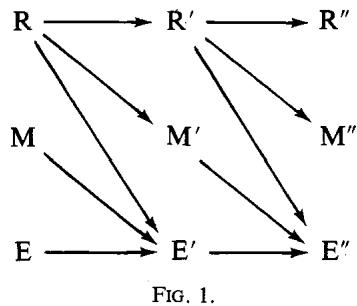
\includegraphics[keepaspectratio]{images/part001_66540ed3.jpg}}

Identifying H(Homgr \(_A\) (C, C')) with Ext (M, M') by the above isomorphism, and likewise for H(Homgr \(_A\) (C', C'')) and H(Homgr \(_A\) (C, C'')), one obtains seven homomorphisms

\[
\operatorname{Ext} _ {\mathbf {A}} \left(\mathrm{M} ^ {\prime}, \mathrm{M} ^ {\prime \prime}\right) \otimes_ {k} \operatorname{Ext} _ {\mathbf {A}} \left(\mathrm{M}, \mathrm{M} ^ {\prime}\right)\rightarrow \operatorname{Ext} _ {\mathbf {A}} \left(\mathrm{M}, \mathrm{M} ^ {\prime \prime}\right).
\]

These seven homomorphisms coincide, and are independent of the choice of resolutions. In particular, they coincide with the homomorphism defined in no. 2, via the triple (I(M), I(M'), I(M')). This follows indeed from the interpretation of the modules H(Homgr (C, C')) as the module of homotopy classes of morphisms of complexes from C to C', and from the fact that if in a diagram of complexes

\[
\begin{array}{c} \mathrm{C} \xrightarrow {f} \mathrm{C} ^ {\prime} \xrightarrow {g} \mathrm{C} ^ {\prime \prime} \\ \alpha \Big \downarrow \qquad \qquad \alpha^ {\prime} \Big \downarrow \qquad \qquad \alpha^ {\prime \prime} \Big \downarrow \\ \mathrm{C} _ {1} \xrightarrow {f _ {1}} \mathrm{C} _ {1} ^ {\prime} \xrightarrow {g _ {1}} \mathrm{C} _ {1} ^ {\prime \prime} \end{array}
\]

\(\alpha'' \circ g\) is homotopic to \(g_1 \circ \alpha'\) and \(\alpha' \circ f\) homotopic to \(f_1 \circ \alpha\) , then \(\alpha'' \circ g \circ f\) is homotopic to \(g_1 \circ f_1 \circ \alpha\) (X, p.~33, prop. 4 and cor.).

In what follows, we shall use, depending on the case, one or another of the seven preceding constructions of composition homomorphisms.

\subsection{The class associated with an exact sequence}

PROPOSITION 1. --- Let (C, d) and (C', d') be two complexes of left A-modules and n, p, q three integers such that \(p \geqslant q\) . For \(p \geqslant i \geqslant q - 1\) , let \(f_i: C_i \to C_{i+n+1}'\) be a homomorphism of A-modules such that \(f_p \circ d = 0\) , \(f_i \circ d = d' \circ f_{i+1}\) for \(p > i \geqslant q - 1\) , and \(d' \circ f_{q-1} = 0\) (see fig.~2).

\pandocbounded{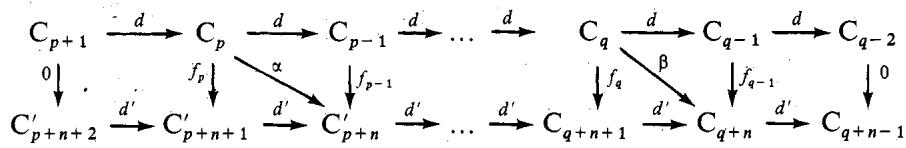
\includegraphics[keepaspectratio]{images/part001_b19b44e0.jpg}}\\
FIG. 2.

Set \(\alpha = f_{p-1} \circ d = d' \circ f_p\) , \(\beta = f_{q-1} \circ d = d' \circ f_q\) , and let \(a\) (resp. \(b\) ) be the graded A-homomorphism of degree \(n\) from C to C' whose only nonzero bihomogeneous component is \(\alpha\) (resp. \(\beta\) ). Then one has \(a \in Z_n(\text{Homgr}_A(C, C'))\) , \(b \in Z_n(\text{Homgr}_A(C, C'))\) and \(a - (-1)^{(n+1)(p-q)} b \in B_n(\text{Homgr}_A(C, C'))\) .

One has \(d' \circ \alpha = d' \circ d' \circ f_p = 0\) , \(\alpha \circ d = f_{p-1} \circ d \circ d = 0\) , hence

\[
a \in Z _ {n} \left(\operatorname{Homgr} _ {\mathrm{A}} \left(\mathrm{C}, \mathrm{C} ^ {\prime}\right)\right);
\]

likewise \(b \in Z_n(\text{Homgr}_A(C, C'))\) . Set \(\varepsilon = (-1)^{n+1}\) . One has, in the complex \(\text{Homgr}_A(C, C')\) the relations

\[
\mathrm{D} f _ {p - 1} = d ^ {\prime} \circ f _ {p - 1} - \varepsilon f _ {p - 1} \circ d = f _ {p - 2} \circ d - \varepsilon \alpha
\]

\[
\mathrm{D} f _ {i} = d ^ {\prime} \circ f _ {i} - \varepsilon f _ {i} \circ d = f _ {i - 1} \circ d - \varepsilon f _ {i} \circ d (p - 1 > i > q)
\]

\[
\mathrm{D} f _ {q} = d ^ {\prime} \circ f _ {q} - \varepsilon f _ {q} \circ d = \beta - \varepsilon f _ {q} \circ d,
\]

hence

\[
\sum_ {i = 1} ^ {p - q} \varepsilon^ {i} D f _ {p - i} = \varepsilon^ {p - q} \beta - \alpha ,
\]

which proves the lemma.

Consider two left A-modules M and N and an exact sequence of A-modules

\[
0 \rightarrow \mathrm{N} \rightarrow \mathrm{R} _ {n} \rightarrow \mathrm{R} _ {n - 1} \rightarrow \dots \rightarrow \mathrm{R} _ {1} \rightarrow \mathrm{M} \rightarrow 0.\tag{4}
\]

By props. 3 and 3 bis of X, p.~49, there exists a commutative diagram:

\begin{enumerate}
\def\labelenumi{(\arabic{enumi})}
\setcounter{enumi}{4}
\tightlist
\item
\end{enumerate}

\pandocbounded{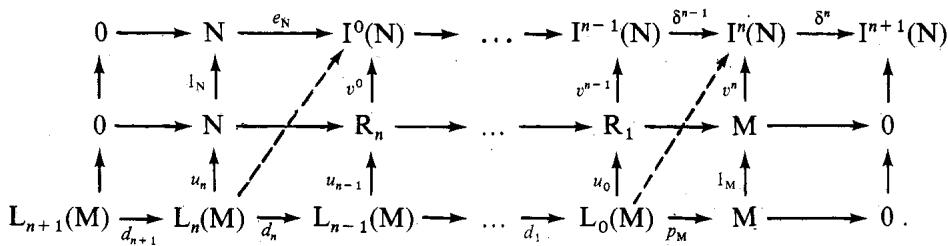
\includegraphics[keepaspectratio]{images/part001_efe78803.jpg}}

Consider the two elements \(b\) and \(a\) of \(\mathrm{Homgr}_{\mathbf{A}}(\mathrm{L}(\mathbf{M}),\mathrm{I}(\mathbf{N}))\) whose only nonzero bihomogeneous components are

\[
b ^ {n} = e _ {\mathrm{N}} \circ u _ {n}: \mathrm{L} _ {n} (\mathrm{M}) \rightarrow \mathrm{I} ^ {0} (\mathrm{N}) \quad \text { and } \quad a ^ {n} = v ^ {n} \circ p _ {\mathrm{M}}: \mathrm{L} _ {0} (\mathrm{M}) \rightarrow \mathrm{I} ^ {n} (\mathrm{N})
\]

respectively.

PROPOSITION 2. --- One has \(a\) , \(b \in Z^n(\text{Homgr}_A (\text{L(M)}, \text{l(N)})\) ). Moreover, the classes \(\overline{a}\) and \(\overline{b}\) of \(a\) and \(b\) in \(\text{H}^n(\text{Homgr}_A (\text{L(M)}, \text{l(N)})) = \text{Ext}_A^n (\text{M}, \text{N})\) depend only on the exact sequence (4) and are equal.

By prop. 1, applied to the two extreme rows of (5) and to the composed vertical arrows, with \(p = n\) , \(q = 0\) , we have \(a\) , \(b \in \mathbf{Z}^{n}(\mathrm{Homgr}_{\mathrm{A}}(\mathrm{l(M)}, \mathrm{L(N)}))\) and

\[
a - b = a - (- 1) ^ {(n + 1) n} b \in \mathrm{B} ^ {n} (\operatorname{Homgr} _ {\mathrm{A}} (\mathrm{L} (\mathrm{M}), \mathrm{I} (\mathrm{N}))).
\]

Since \(a\) (resp. \(b\) ) is independent of the choice of \(u\) (resp. \(v\) ), the element \(\overline{a} = \overline{b}\) of \(\mathrm{Ext}_{\mathbf{A}}^{n}\) (M, N) is independent of the choice of morphisms \(u\) and \(v\) , whence the proposition.

DEFINITION 1. --- The element \(\theta\) of \(\operatorname{Ext}_{\mathbf{A}}^{n}(\mathbf{M}, \mathbf{N})\) defined by \(\theta = (-1)^{n(n+1)/2} \overline{a} = (-1)^{n(n+1)/2} \overline{b}\) is called the class associated with the exact sequence (4) .

Remarks. --- 1) Let (P, p) be a projective resolution of M. By X, p.~49, prop. 3, there exists a commutative diagram

\[
\begin{array}{c} 0 \longrightarrow \mathrm{N} \longrightarrow \mathrm{R} _ {n} \longrightarrow \dots \longrightarrow \mathrm{R} _ {1} \longrightarrow \mathrm{M} \longrightarrow 0 \\ \tilde {u} _ {n} \uparrow \quad \tilde {u} _ {n - 1} \uparrow \quad \tilde {u} _ {0} \uparrow \quad \uparrow_ {\mathrm{M}} \\ \mathrm{P} _ {n} \longrightarrow \mathrm{P} _ {n - 1} \longrightarrow \dots \longrightarrow \mathrm{P} _ {0} \xrightarrow {p} \mathrm{M} \longrightarrow 0. \end{array}
\]

With the notations of § 6, θ is the image under φ(P, N) of the homotopy class of the morphism P → N defined by \((-1)^{n(n+1)/2} \tilde{u}_{n}\) . Similarly, if \((e, E)\) is an injective resolution of N, there exists a commutative diagram

\[
\begin{array}{c} 0 \longrightarrow \mathrm{N} \longrightarrow \mathrm{E} ^ {0} \longrightarrow \dots \longrightarrow \mathrm{E} ^ {n - 1} \longrightarrow \mathrm{E} ^ {n} \\ 1 _ {\mathrm{N}} \uparrow \quad \tilde {v} ^ {0} \uparrow \quad \quad \quad \quad \quad \quad \quad \quad \quad \quad \quad \quad \quad \quad \quad \quad \quad \quad \quad \quad \quad \quad \quad \quad 0 \longrightarrow \mathrm{N} \longrightarrow \mathrm{R} _ {n} \longrightarrow \dots \longrightarrow \mathrm{R} _ {1} \longrightarrow \mathrm{M} \longrightarrow 0. \end{array}
\]

and \(\theta\) is the image under \(\varphi(\mathbf{M},\mathbf{E})\) of the homotopy class of the morphism \(\mathbf{M}\to\mathbf{E}\) defined by \((-1)^{n(n+1)/2}v^{n}\) . This follows from the construction of \(\theta\) and definitions of \(\varphi(\mathbf{P},\mathbf{N})\) and \(\varphi(\mathbf{M},\mathbf{E})\) .

\begin{enumerate}
\def\labelenumi{\arabic{enumi})}
\setcounter{enumi}{1}
\tightlist
\item
  When \(n = 0\) , the exact sequence (4) is written \(0 \to \mathbf{N} \xrightarrow{f} \mathbf{M} \to 0\) , and the associated class is \(f^{-1} \in \operatorname{Hom}_{\mathbf{A}}(\mathbf{M}, \mathbf{N}) = \operatorname{Ext}_{\mathbf{A}}^{0}(\mathbf{M}, \mathbf{N})\) .
\end{enumerate}

\subsection{Properties of the class associated with an exact sequence}

PROPOSITION 3. — Let

\begin{enumerate}
\def\labelenumi{(\arabic{enumi})}
\setcounter{enumi}{5}
\tightlist
\item
\end{enumerate}

\[
0 \rightarrow \mathrm{P} \rightarrow \mathrm{S} _ {m} \rightarrow \mathrm{S} _ {m - 1} \rightarrow \dots \rightarrow \mathrm{S} _ {1} \stackrel {\lambda_ {n}} {\rightarrow} \mathrm{N} \rightarrow 0\tag{7}
\]

\[
0 \rightarrow \mathrm{N} \xrightarrow {\mu} \mathrm{R} _ {n} \rightarrow \mathrm{R} _ {n - 1} \rightarrow \dots \rightarrow \mathrm{R} _ {1} \rightarrow \mathrm{M} \rightarrow 0
\]

two exact sequences of left A-modules of respective classes \(\theta\in\mathrm{Ext}_{\mathbf{A}}^{m}(\mathbf{N},\mathbf{P})\) and \(\theta^{\prime}\in\mathrm{Ext}_{\mathbf{A}}^{n}(\mathbf{M},\mathbf{N})\) . The class in \(\mathrm{Ext}_{\mathbf{A}}^{m+n}(\mathbf{M},\mathbf{P})\) associated with the exact sequence

\[
0 \to \mathrm{P} \to \mathrm{S} _ {m} \to \dots \to \mathrm{S} _ {1} \xrightarrow {\mu \circ \lambda} \mathrm{R} _ {n} \to \dots \to \mathrm{R} _ {1} \to \mathrm{M} \to 0\tag{8}
\]

is the composition product \(\theta\circ\theta'\) .

Let us choose commutative diagrams

\[
\begin{array}{c} 0 \longrightarrow \mathrm{P} \longrightarrow \mathrm{I} ^ {0} (\mathrm{P}) \longrightarrow \dots \longrightarrow \mathrm{I} ^ {m - 1} (\mathrm{P}) \xrightarrow {\delta_ {\mathrm{P}} ^ {m - 1}} \mathrm{I} ^ {m} (\mathrm{P}) \\ 0 \longrightarrow \mathrm{P} \longrightarrow \mathrm{S} _ {m} \longrightarrow \dots \longrightarrow \mathrm{S} _ {1} \xrightarrow {\lambda} \mathrm{N} \longrightarrow 0, \end{array}
\]

\[
\begin{array}{c c c c c c c c c c c c} 0 \longrightarrow & \mathrm{N} & \stackrel {{e _ {\mathrm{N}}}} {{\longrightarrow}} & \mathrm{I} ^ {0} (\mathrm{N}) & \longrightarrow & \dots & \longrightarrow & \mathrm{I} ^ {n - 1} (\mathrm{N}) & \longrightarrow & \mathrm{I} ^ {n} (\mathrm{N}) \\ & \uparrow_ {1 _ {\mathrm{N}}} & & v ^ {0} \uparrow & & & & v ^ {n - 1} \uparrow & & v ^ {n} \uparrow \\ 0 \longrightarrow & \mathrm{N} & \stackrel {{\mu}} {{\longrightarrow}} & \mathrm{R} _ {n} & \longrightarrow & \dots & \longrightarrow & \mathrm{R} _ {1} & \longrightarrow & \mathrm{M} & \longrightarrow & 0. \end{array}
\]

Since \(\mathrm{I}^{m}(\mathrm{P})\) is injective, there exists a homomorphism \(h^{0}: \mathrm{I}^{0}(\mathrm{N}) \to \mathrm{I}^{m}(\mathrm{P})\) such that \(w^{m} = h^{0} \circ e_{N}\) ; by X, p.~49, prop. 3 bis, \(h^{0}\) extends to a morphism of complexes \(h: \mathrm{I}(\mathrm{N}) \to \mathrm{I}(\mathrm{P})(-m)\) . Then \(w^{m} = h^{0} \circ e_{N} = h^{0} \circ v^{0} \circ \mu\) , hence

\[
\delta_ {1} ^ {m - 1} \circ w ^ {m - 1} = w ^ {m} \circ \lambda = h ^ {0} \circ v ^ {0} \circ (\mu \circ \lambda),
\]

and the following diagram is commutative:

\[
\begin{array}{l}0 \longrightarrow \mathrm{P} \longrightarrow \mathrm{I} ^ {0} (\mathrm{P}) \longrightarrow \dots \longrightarrow \mathrm{I} ^ {m - 1} (\mathrm{P}) \longrightarrow \mathrm{I} ^ {m} (\mathrm{P}) \longrightarrow \mathrm{I} ^ {m + 1} (\mathrm{P}) \longrightarrow \dots \longrightarrow \mathrm{I} ^ {m + n} (\mathrm{P})\\0 \longrightarrow \mathrm{P} \longrightarrow \mathrm{S} _ {m} \longrightarrow \dots \longrightarrow \mathrm{S} _ {1} \underset {\mu \circ \lambda} {\longrightarrow} \mathrm{R} _ {n} \longrightarrow \mathrm{R} _ {n - 1} \longrightarrow \dots \longrightarrow \mathrm{M} \rightarrow 0\end{array}
\]

where \(t^0 = h^0 \circ v^0\) , \(t^1 = (-1)^m h^1 \circ v^1, \ldots, t^i = (-1)^{mi} h^i \circ v^i, \ldots, t^n = (-1)^{mn} h^n \circ v^n\) . The class \(\theta\) associated with (6) is that of \((-1)^{m(m+1)/2} w^m \in \text{Homgr}_A^m(\mathbf{N}, \mathbf{l}(\mathbf{P}))\) , hence corresponds under the isomorphism \(a_{\mathbf{N},\mathbf{P}}\) to the class of \((-1)^{m(m+1)/2} h \in \text{Homgr}_A^m(\mathbf{l}(\mathbf{N}), \mathbf{l}(\mathbf{P}))\) ; the class \(\theta'\) associated with (7) is that of \((-1)^{n(n+1)/2} v^n \in \text{Homgr}_A^m(\mathbf{M}, \mathbf{l}(\mathbf{N}))\) , the class associated with (8) is that of \((-1)^{(m+n)(m+n+1)/2} t^n \in \text{Homgr}_{m+n}^m(\mathbf{M}, \mathbf{l}(\mathbf{P}))\) whence the conclusion, by the definition of the composition product (X, p.~114) and the formula

\[
m (m + 1) / 2 + n (n + 1) / 2 = (m + n) (m + n + 1) / 2 - m n.
\]

\begin{enumerate}
\def\labelenumi{\arabic{enumi}.}
\setcounter{enumi}{3}
\tightlist
\item
  --- Consider a commutative diagram of A-modules with exact
\end{enumerate}

rows

\pandocbounded{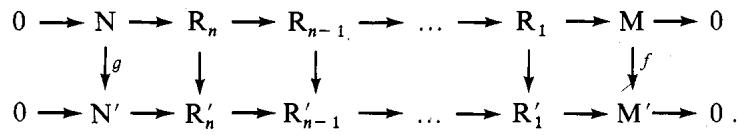
\includegraphics[keepaspectratio]{images/part001_b790ce53.jpg}}

Let θ (resp. θ′) be the class of the first (resp. second) row in

\[
\operatorname{Ext} _ {\mathbf {A}} ^ {n} (\mathbf {M}, \mathbf {N}) \quad \left(\text { resp.   } \operatorname{Ext} _ {\mathbf {A}} ^ {n} (\mathbf {M} ^ {\prime}, \mathbf {N} ^ {\prime})\right).
\]

In \(\operatorname{Ext}_{\mathbf{A}}^{n}(\mathbf{M}, \mathbf{N}')\) , one has \(\theta' \circ f = g \circ \theta\) .

Indeed, consider a commutative diagram

\pandocbounded{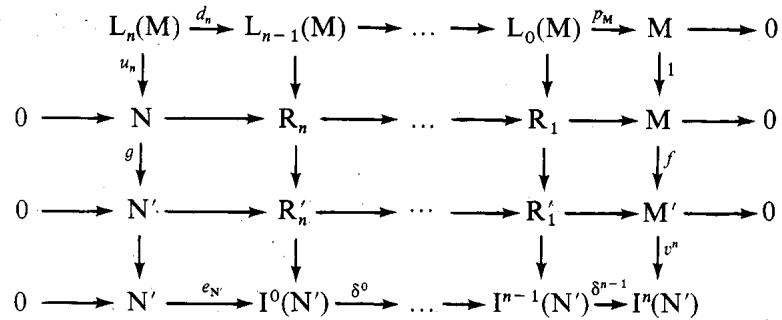
\includegraphics[keepaspectratio]{images/part001_126cf8d3.jpg}}

By definition \(\theta' \circ f\) is the class of \((-1)^{n(n+1)/2} v^n \circ f \circ p_M \in \text{Homgr}^n (\text{L(M)}, \text{I(N')})\) , whereas \(g \circ \theta\) is the class of \((-1)^{n(n+1)/2} e_{N'} \circ g \circ u_n\) . By Lemma 1, applied to the two extreme rows of the diagram, these two classes are equal.

COROLLARY 1. --- Consider a commutative diagram with exact rows

\[
\begin{array}{c c c c c c c c} 0 \longrightarrow & \mathrm{N} \longrightarrow & \mathrm{R} _ {n} \longrightarrow & \dots & \longrightarrow & \mathrm{R} _ {1} \longrightarrow & \mathrm{M} \longrightarrow & 0 \\ & ^ {1} \downarrow & & & \downarrow & & ^ {1} \downarrow \\ 0 \longrightarrow & \mathrm{N} \longrightarrow & \mathrm{R} _ {n} ^ {\prime} \longrightarrow & \dots & \longrightarrow & \mathrm{R} _ {1} ^ {\prime} \longrightarrow & \mathrm{M} \longrightarrow & 0; \end{array}
\]

the two rows of the diagram have the same associated class in \(\operatorname{Ext}_{\mathbf{A}}^{n}(\mathbf{M},\mathbf{N})\) .

COROLLARY 2. --- Let

\[
0 \rightarrow \mathrm{N} \xrightarrow {f _ {n - 1}} \mathrm{R} _ {n} \xrightarrow {f _ {n}} \mathrm{R} _ {n - 1} \rightarrow \dots \xrightarrow {f _ {2}} \mathrm{R} _ {1} \xrightarrow {f _ {1}} \mathrm{M} \rightarrow 0
\]

be an exact sequence, \(\theta\in\mathrm{Ext}_{\mathbf{A}}^{n}(\mathbf{M},\mathbf{N})\) the associated class, \(a_{1},\ldots,a_{n+1}\) invertible elements of \(k\) . The class associated with the exact sequence

\[
0 \rightarrow \mathrm{N} \xrightarrow {a _ {n + 1} f _ {n + 1}} \mathrm{R} _ {n} \xrightarrow {a _ {n} f _ {n}} \mathrm{R} _ {n - 1} \rightarrow \dots \xrightarrow {a _ {2} f _ {2}} \mathrm{R} _ {1} \xrightarrow {a _ {1} f _ {1}} \mathrm{M} \rightarrow 0
\]

is \((a_{1}^{-1}a_{2}^{-1}\dots a_{n + 1}^{-1})\theta .\)

Indeed, we have a commutative diagram

\[
\begin{array}{c} 0 \longrightarrow \mathrm{N} \xrightarrow {a _ {n + 1} f _ {n + 1}} \mathrm{R} _ {n} \longrightarrow \dots \longrightarrow \mathrm{R} _ {2} \xrightarrow {a _ {2} f _ {2}} \mathrm{R} _ {1} \xrightarrow {a _ {1} f _ {1}} \mathrm{M} \longrightarrow 0 \\ \Biggl \downarrow a _ {1} \dots a _ {n + 1} \quad \Biggl \downarrow a _ {1} \dots a _ {n} \quad \Biggl \downarrow a _ {1} a _ {2} \quad \Biggl \downarrow a _ {1} \quad \Biggl \downarrow 1 \\ 0 \longrightarrow \mathrm{N} \xrightarrow {f _ {n + 1}} \mathrm{R} _ {n} \longrightarrow \dots \longrightarrow \mathrm{R} _ {2} \xrightarrow {f _ {2}} \mathrm{R} _ {1} \xrightarrow {f _ {1}} \mathrm{M} \longrightarrow 0. \end{array}
\]

and we apply the proposition.

COROLLARY 3. --- Let \(0 \to \mathbf{N} \xrightarrow{f_{n+1}} \mathbf{R}_{n} \xrightarrow{f_{n}} \cdots \to \mathbf{R}_{1} \xrightarrow{f_{1}} \mathbf{M} \to 0\) be an exact sequence, \(\theta\) its class in \(\operatorname{Ext}_{\mathbf{A}}^{n}(\mathbf{M}, \mathbf{N})\) , \(u: \mathbf{M}' \to \mathbf{M}\) and \(v: \mathbf{N} \to \mathbf{N}'\) be two homomorphisms of A-modules.

\begin{enumerate}
\def\labelenumi{\alph{enumi})}
\tightlist
\item
  The element \(v \circ \theta\) of \(\operatorname{Ext}_{\mathbf{A}}^{n}(\mathbf{M}, \mathbf{N}')\) is equal to the class of the exact sequence
\end{enumerate}

\[
0 \rightarrow \mathrm{N} ^ {\prime} \xrightarrow {f _ {n + 1} ^ {\prime}} \mathrm{R} _ {n} ^ {\prime} \xrightarrow {f _ {n} ^ {\prime}} \mathrm{R} _ {n - 1} \xrightarrow {f _ {n - 1}} \dots \rightarrow \mathrm{R} _ {1} \rightarrow \mathrm{M} \rightarrow 0,
\]

where \(R_{n}^{\prime}\) is the A-module quotient of \(R_{n} \oplus N^{\prime}\) by the submodule formed by the pairs \((f_{n+1}(x), -v(x))\) for \(x \in N\) , and where \(f_{n+1}^{\prime}\) (resp. \(f_{n}^{\prime}\) ) is deduced from the canonical injection (resp. from \((f_{n}, 0)\) ) by passing to quotients.

\begin{enumerate}
\def\labelenumi{\alph{enumi})}
\setcounter{enumi}{1}
\tightlist
\item
  The element \(\theta \circ u\) of \(\operatorname{Ext}_{\mathbf{A}}^{n}(\mathbf{M}^{\prime}, \mathbf{N})\) is the class of the exact sequence
\end{enumerate}

\[
0 \rightarrow \mathrm{N} \rightarrow \mathrm{R} _ {n} \rightarrow \dots \rightarrow \mathrm{R} _ {2} \xrightarrow {f _ {2} ^ {\prime \prime}} \mathrm{R} _ {1} ^ {\prime} \xrightarrow {f _ {1} ^ {\prime \prime}} \mathrm{M} ^ {\prime} \rightarrow 0,
\]

where \(R_{1}^{\prime}\) is the fiber product \(R_{1} \times_{M} M^{\prime}\) , that is to say (I, p.~44) the submodule of \(R_{1} \times M^{\prime}\) formed by the pairs \((x, y)\) such that \(f_{1}(x) = u(y)\) , and where \(f_{2}^{\prime\prime}\) (resp. \(f_{1}^{\prime\prime}\) ) is deduced from \((f_{2}, 0)\) (resp. from the second projection).

Let us prove for example \(a\) ). Let \(z\) be an element of \(\mathbf{R}_{n}^{\prime}\) such that \(f_{n}^{\prime}(z)=0\) ; if \(z\) is the class of a pair \((x,y)\) , with \(x\in\mathbf{R}_{n},y\in\mathbf{N}^{\prime}\) , we have \(f_{n}(x)=0\) so that there exists an element \(t\in\mathbf{N}\) such that \(x=f_{n+1}(t)\) . We then have \(z=f_{n+1}^{\prime}(y+v(t))\) which proves that \(\operatorname{Ker} f_{n}^{\prime}=\operatorname{Im} f_{n+1}^{\prime}\) . The injectivity of \(f_{n+1}^{\prime}\) follows from that of the \(f_{n+1}\) .

Let \(j: \mathbf{R}_{n} \to \mathbf{R}_{n}^{\prime}\) be the homomorphism deduced from the canonical injection; we have a commutative diagram of exact sequences:

\[
\begin{array}{c} 0 \longrightarrow \mathrm{N} \xrightarrow {f _ {n + 1}} \mathrm{R} _ {n} \xrightarrow {f _ {n}} \mathrm{R} _ {n - 1} \longrightarrow \dots \longrightarrow \mathrm{M} \longrightarrow 0 \\ \Biggl \downarrow v \quad \Biggl \downarrow j \quad \Biggl \downarrow 1 \\ 0 \longrightarrow \mathrm{N} ^ {\prime} \xrightarrow {f _ {n + 1} ^ {\prime}} \mathrm{R} _ {n} ^ {\prime} \xrightarrow {f _ {n} ^ {\prime}} \mathrm{R} _ {n - 1} \longrightarrow \dots \longrightarrow \mathrm{M} \longrightarrow 0; \end{array}
\]

assertion a) then follows from the proposition.

The proof of \(b\) is analogous.

Remark. --- Let \(\theta\in\mathrm{Ext}_{\mathbf{A}}^{n}(\mathbf{M},\mathbf{N})\) , resp. \(\theta^{\prime}\in\mathrm{Ext}_{\mathbf{A}}^{n}(\mathbf{M}^{\prime},\mathbf{N}^{\prime})\) , be the class of an exact sequence

\[
0 \rightarrow \mathrm{N} \xrightarrow {f _ {n + 1}} \mathrm{R} _ {n} \rightarrow \dots \rightarrow \mathrm{R} _ {1} \xrightarrow {f _ {1}} \mathrm{M} \rightarrow 0,
\]

\[
\text { resp. } 0 \to \mathrm{N} ^ {\prime} \xrightarrow {f _ {n + 1} ^ {\prime}} \mathrm{R} _ {n} ^ {\prime} \to \dots \to \mathrm{R} _ {1} ^ {\prime} \xrightarrow {f _ {1} ^ {\prime}} \mathrm{M} ^ {\prime} \to 0.
\]

Let \(i_{\mathbf{N}}, i_{\mathbf{N}'}\) , be the canonical injections of \(\mathbf{N}\) and \(\mathbf{N}'\) into \(\mathbf{N} \oplus \mathbf{N}'\) , \(q_{\mathbf{M}}\) , \(q_{\mathbf{M}'}\) , the projections of \(\mathbf{M} \oplus \mathbf{M}'\) onto \(\mathbf{M}\) and \(\mathbf{M}'\) . Consider the homomorphism

\[
m = \operatorname{Ext} \left(q _ {\mathbf {M}}, i _ {\mathbf {N}}\right) \oplus \operatorname{Ext} \left(q _ {\mathbf {M} ^ {\prime}}, i _ {\mathbf {N} ^ {\prime}}\right)
\]

of \(\operatorname{Ext}_{\mathbf{A}}(\mathbf{M},\mathbf{N})\oplus \operatorname{Ext}_{\mathbf{A}}(\mathbf{M}^{\prime},\mathbf{N}^{\prime})\) to \(\operatorname{Ext}_{\mathbf{A}}(\mathbf{M}\oplus \mathbf{M}^{\prime},\mathbf{N}\oplus \mathbf{N}^{\prime}\) . The element

\[
m (\theta , \theta^ {\prime}) = i _ {\mathrm{N}} \circ \theta \circ q _ {\mathrm{M}} + i _ {\mathrm {N^ {\prime}}} \circ \theta^ {\prime} \circ q _ {\mathrm {M^ {\prime}}}
\]

is the class of the exact sequence

\[
0 \rightarrow \mathrm{N} \oplus \mathrm{N} ^ {\prime} \xrightarrow {f _ {n + 1} \oplus f _ {n - 1} ^ {\prime}} \mathrm{R} _ {n} \oplus \mathrm{R} _ {n} ^ {\prime} \rightarrow \dots \rightarrow \mathrm{R} _ {1} \oplus \mathrm{R} _ {1} ^ {\prime} \xrightarrow {f _ {1} \oplus f _ {1} ^ {\prime}} \mathrm{M} \oplus \mathrm{M} ^ {\prime} \rightarrow 0.
\]

Indeed, if one denotes this class by \(\theta''\) , it follows from prop. 4 that one has

\[
\theta^ {\prime \prime} \circ i _ {\mathrm{M}} = i _ {\mathrm{N}} \circ \theta = m (\theta , \theta^ {\prime}) \circ i _ {\mathrm{M}} \quad \text {and} \quad \theta^ {\prime \prime} \circ i _ {\mathrm{M} ^ {\prime}} = i _ {\mathrm{N} ^ {\prime}} \circ \theta = m (\theta , \theta^ {\prime}) \circ i _ {\mathrm{M} ^ {\prime}};
\]

according to X, p.~89, prop. 7, this implies \(\theta'' = m(\theta, \theta')\) .

\subsection{\texorpdfstring{Relation between exact sequences and elements of Ext \(_{A}\) (M, N)}{Relation between exact sequences and elements of Ext \_\{A\} (M, N)}}

THEOREM 1. --- Let n be an integer ≥1, and M and N two A-modules.

\begin{enumerate}
\def\labelenumi{\alph{enumi})}
\item
  Every element of Ext \(_{A}^{n}\) (M, N) is the class of an exact sequence (X, p.~117, def. 1).
\item
  Let \(0 \to \mathbf{N} \xrightarrow{f_{n+1}} \mathbf{R}_n \xrightarrow{f_n} \ldots \to \mathbf{R}_1 \xrightarrow{f_1} \mathbf{M} \to 0\)
\end{enumerate}

and

\[
0 \rightarrow \mathrm{N} \xrightarrow {f _ {n + 1} ^ {\prime}} \mathrm{R} _ {n} ^ {\prime} \xrightarrow {f _ {n} ^ {\prime}} \dots \rightarrow \mathrm{R} _ {1} ^ {\prime} \xrightarrow {f _ {1} ^ {\prime}} \mathrm{M} \rightarrow 0
\]

of exact sequences, \(\theta\) and \(\theta'\) the associated classes. The following conditions are equivalent:

\begin{enumerate}
\def\labelenumi{(\roman{enumi})}
\item
  \(\theta = \theta^{\prime}\) ;
\item
  there exists a commutative diagram with exact rows:
\end{enumerate}

\[
\begin{array}{c} 0 \longrightarrow \mathrm{N} \xrightarrow {f _ {n + 1}} \mathrm{R} _ {n} \longrightarrow \dots \longrightarrow \mathrm{R} _ {1} \xrightarrow {f _ {1}} \mathrm{M} \longrightarrow 0 \\ 0 \longrightarrow \mathrm{N} \longrightarrow \mathrm{R} _ {n} ^ {\prime \prime} \longrightarrow \dots \longrightarrow \mathrm{R} _ {1} ^ {\prime} \longrightarrow \mathrm{M} \longrightarrow 0 \\ 0 \longrightarrow \mathrm{N} \xrightarrow {f _ {n + 1} ^ {\prime}} \mathrm{R} _ {n} ^ {\prime} \longrightarrow \dots \longrightarrow \mathrm{R} _ {1} ^ {\prime} \xrightarrow {f _ {1} ^ {\prime}} \mathrm{M} \longrightarrow 0; \end{array}
\]

\begin{enumerate}
\def\labelenumi{(\roman{enumi})}
\setcounter{enumi}{2}
\tightlist
\item
  there exists a commutative diagram with exact rows:
\end{enumerate}

\[
\begin{array}{c} 0 \longrightarrow \mathrm{N} \xrightarrow {f _ {n + 1}} \mathrm{R} _ {n} \longrightarrow \dots \longrightarrow \mathrm{R} _ {1} \xrightarrow {f _ {1}} \mathrm{M} \longrightarrow 0 \\ 0 \longrightarrow \mathrm{N} \longrightarrow \mathrm{R} _ {n} ^ {\prime \prime} \longrightarrow \dots \longrightarrow \mathrm{R} _ {1} ^ {\prime \prime} \longrightarrow \mathrm{M} \longrightarrow 0 \\ 0 \longrightarrow \mathrm{N} \xrightarrow {f _ {n + 1} ^ {\prime}} \mathrm{R} _ {n} ^ {\prime} \longrightarrow \dots \longrightarrow \mathrm{R} _ {1} ^ {\prime} \xrightarrow {f _ {1} ^ {\prime}} \mathrm{M} \longrightarrow 0. \end{array}
\]

Let us prove \(a\) ). Let \(\alpha \in \operatorname{Ext}_{\mathbf{A}}^{n}(\mathbf{M}, \mathbf{N})\) , and let \(\mathbf{P}\) be a projective resolution of \(\mathbf{M}\) . Let \(a: \mathrm{P}(n) \to \mathbf{N}\) be a morphism of complexes representing \(\alpha\) ; its unique nonzero component is an A-homomorphism \(u: \mathrm{P}_{n} \to \mathbf{N}\) which satisfies \(u \circ d_{n+1} = 0\) , hence factors through \(u = \overline{u} \circ \delta_{n}\) , where \(\delta_{n}: \mathrm{P}_{n} \to \dot{\mathbf{Z}}_{n-1}\) is the map induced by \(d_{n}\) (we set \(Z_{n-1} = \operatorname{Im} d_{n}\) ) and \(\overline{u}\) is an A-homomorphism of \(Z_{n-1}\) to \(\mathbf{N}\) . By Remark 1, p.~117, the class \(\theta \in \operatorname{Ext}_{\mathbf{A}}^{n}(\mathbf{M}, Z_{n-1})\) of the exact sequence

\[
0 \rightarrow Z _ {n - 1} \rightarrow P _ {n - 1} \rightarrow \dots \rightarrow P _ {0} \rightarrow M \rightarrow 0
\]

is equal to the homotopy class of the morphism \((-1)^{n(n + 1) / 2}\delta_n\) . We therefore have

\[
\alpha = (- 1) ^ {n (n + 1) / 2} \overline {{{u}}} \circ \theta ,
\]

which, according to Cor. 3, p.~120, allows one to represent α as the class of an exact sequence.

It follows from cor. 1 of X, p.~120 that (ii) \(\Rightarrow\) (i) and that (iii) \(\Rightarrow\) (i). Suppose (i) is satisfied, and let P be a projective resolution of M. There exists a commutative diagram

\[
\begin{array}{c} 0 \longrightarrow \mathrm{N} \xrightarrow {f _ {n + 1}} \mathrm{R} _ {n} \longrightarrow \mathrm{R} _ {n - 1} \longrightarrow \dots \longrightarrow \mathrm{R} _ {1} \longrightarrow \mathrm{M} \longrightarrow 0 \\ u _ {n} \uparrow \quad \uparrow u _ {n - 1} \quad \uparrow u _ {n - 2} \quad \uparrow \quad \uparrow_ {\mathrm{I} _ {\mathrm{M}}} \\ \mathrm{P} _ {n} \xrightarrow {d _ {n}} \mathrm{P} _ {n - 1} \longrightarrow \mathrm{P} _ {n - 2} \longrightarrow \dots \longrightarrow \mathrm{P} _ {0} \longrightarrow \mathrm{M} \longrightarrow 0 \\ u _ {n} ^ {\prime} \downarrow \quad \downarrow u _ {n - 1} ^ {\prime} \quad \downarrow u _ {n - 2} ^ {\prime} \quad \downarrow \quad \downarrow_ {\mathrm{I} _ {\mathrm{M}}} \\ 0 \longrightarrow \mathrm{N} \xrightarrow {f _ {n + 1}} \mathrm{R} _ {n} ^ {\prime} \longrightarrow \mathrm{R} _ {n - 1} ^ {\prime} \longrightarrow \dots \longrightarrow \mathrm{R} _ {1} ^ {\prime} \longrightarrow \mathrm{M} \longrightarrow 0. \end{array}
\]

The morphisms of \(\mathrm{P}(n)\) to \(\mathbf{N}\) defined by \(u_{n}\) and \(u_{n}^{\prime}\) are homotopic, since they both belong to the class \((-1)^{n(n + 1) / 2}\theta\) , hence \(u_{n}^{\prime} - u_{n}\) is of the form \(w\circ d_n\) , where \(w:\mathrm{P}_{n - 1}\to \mathrm{N}\) is an A-homomorphism. By replacing \(u_{n - 1}^{\prime}\) by \(u_{n - 1}^{\prime} - f_{n + 1}^{\prime}\circ w\) and \(u_{n}^{\prime}\) by \(u_{n}\) one reduces to the case where \(u_{n} = u_{n}^{\prime}\) . This allows one to construct a new commutative diagram with exact rows:

\[
\begin{array}{c c c c c c c} 0 \longrightarrow \mathrm{N} \longrightarrow \mathrm{R} _ {n} \longrightarrow \mathrm{R} _ {n - 1} \longrightarrow \dots \longrightarrow \mathrm{R} _ {1} \longrightarrow \mathrm{M} \longrightarrow 0 \\ 1 _ {\mathrm{N}} \uparrow & \uparrow v & \uparrow u _ {n - 2} & \uparrow & \uparrow^ {1 _ {\mathrm{M}}} \\ 0 \longrightarrow \mathrm{N} \longrightarrow \mathrm{N} ^ {\prime} \longrightarrow \mathrm{P} _ {n - 2}. \longrightarrow \dots \longrightarrow \mathrm{P} _ {0} \longrightarrow \mathrm{M} \longrightarrow 0 \\ 1 _ {\mathrm{N}} \downarrow & \downarrow v ^ {\prime} & \downarrow u _ {n - 2} ^ {\prime} & \downarrow & \downarrow^ {1 _ {\mathrm{M}}} \\ 0 \longrightarrow \mathrm{N} \longrightarrow \mathrm{R} _ {n} ^ {\prime} \longrightarrow \mathrm{R} _ {n - 1} ^ {\prime} \longrightarrow \dots \longrightarrow \mathrm{R} _ {1} ^ {\prime} \longrightarrow \mathrm{M} \longrightarrow 0 \end{array}
\]

where \(\mathbf{N}'\) is the quotient of \(\mathbf{P}_{n-1} \oplus \mathbf{N}\) by the submodule formed by the pairs \((d_n(x), -u_n(x))\) for \(x \in \mathbf{P}_n\) , and where \(v\) (resp. \(v'\) ) is defined by passing to the quotient from the map \(u_{n-1} \oplus f_{n+1}\) (resp. \(u_{n-1}' \oplus f_{n+1}'\) ). Condition (ii) is therefore satisfied.

Suppose again that condition (i) is satisfied, and let E be an injective resolution of N. There exists a commutative diagram

\[
\begin{array}{c c c c c c c} 0 \longrightarrow \mathrm{N} \longrightarrow \mathrm{R} _ {n} \longrightarrow & \dots \longrightarrow \mathrm{R} _ {1} \longrightarrow \mathrm{M} \longrightarrow & 0 \\ 1 _ {\mathrm{N}} \Big \downarrow & \Big \downarrow v _ {0} & v _ {n - 1} \Big \downarrow & \Big \downarrow v _ {n} \\ 0 \longrightarrow \mathrm{N} ^ {\prime} \longrightarrow \mathrm{E} ^ {0} \stackrel {{\delta^ {0}}} {{\longrightarrow}} & \dots \longrightarrow \mathrm{E} ^ {n - 1} \stackrel {{\delta^ {n - 1}}} {{\longrightarrow}} \mathrm{E} ^ {n} \\ 1 _ {\mathrm{N}} \Big \uparrow & \Big \uparrow v _ {0} ^ {\prime} & v _ {n - 1} ^ {\prime} \Big \uparrow & \Big \uparrow v _ {n} ^ {\prime} \\ 0 \longrightarrow \mathrm{N} \longrightarrow \mathrm{R} _ {n} ^ {\prime} \longrightarrow & \dots \longrightarrow \mathrm{R} _ {1} ^ {\prime} \longrightarrow & \mathrm{M} \longrightarrow & 0 \end{array}
\]

and one shows as above that one may assume \(v_{n}^{\prime}=v_{n}\) . We then have a commutative diagram with exact rows

\[
\begin{array}{c c c c c c c c} 0 \longrightarrow N \longrightarrow R _ {n} \longrightarrow \dots \longrightarrow R _ {2} \longrightarrow R _ {1} \longrightarrow M \longrightarrow 0 \\ \downarrow^ {1 _ {N}} & \downarrow & & \downarrow & \downarrow & \downarrow^ {1 _ {M}} \\ 0 \longrightarrow N \longrightarrow E ^ {0} \longrightarrow \dots \longrightarrow E ^ {n - 2} \longrightarrow M ^ {\prime} \longrightarrow M \longrightarrow 0 \\ \uparrow^ {1 _ {N}} & \uparrow & & \uparrow & \uparrow & \uparrow^ {1 _ {M}} \\ 0 \longrightarrow N \longrightarrow R _ {n} ^ {\prime} \longrightarrow \dots \longrightarrow R _ {2} ^ {\prime} \longrightarrow R _ {1} ^ {\prime} \longrightarrow M \longrightarrow 0 \end{array}
\]

with \(\mathbf{M}' = \mathbf{M} \times_{\mathrm{R}_{1}} \mathbf{E}_{n-1}\) (cf. X, p. 120, cor. 3, b)). Condition (iii) is therefore satisfied, which completes the proof of the theorem.

Remark 1. --- If the ring A is Noetherian, and if the A-modules M and N are finitely generated, it follows from the proof of a) that every element of Ext \(_{A}^{n}\) (M, N) is the class associated with an exact sequence 0 → N → R \(_{n}\) → \ldots{} → R \(_{1}\) → M → 0 where the R \(_{i}\) are finitely generated.

COROLLARY. --- Let \(0 \to \mathbf{N} \xrightarrow{f} \mathbf{R} \xrightarrow{g} \mathbf{M} \to 0\) and \(0 \to \mathbf{N} \xrightarrow{f'} \mathbf{R}' \xrightarrow{g'} \mathbf{M} \to 0\) be two exact sequences, \(\theta\) and \(\theta'\) the associated classes in \(\operatorname{Ext}^1(\mathbf{M}, \mathbf{N})\) . For \(\theta = \theta'\) , it is necessary and sufficient that there exist an A-homomorphism \(h: \mathbf{R} \to \mathbf{R}'\) making the diagram

\[
\begin{array}{c} \mathsf {R} \\ \mathsf {N} \\ \mathsf {f ^ {\prime}} \end{array} \begin{array}{c} \mathsf {f} \\ \mathsf {h} \\ \mathsf {R ^ {\prime}} \end{array} \begin{array}{c} \mathsf {g} \\ \mathsf {M} \\ \mathsf {g ^ {\prime}} \end{array}
\]

commutative. Such a homomorphism is necessarily an isomorphism.

The condition is sufficient by cor. 1 of prop. 4. If \(\theta = \theta'\) , we have a commutative diagram with exact rows:

\[
\begin{array}{c} 0 \longrightarrow \mathrm{N} \longrightarrow \mathrm{R} \longrightarrow \mathrm{M} \longrightarrow 0 \\ \uparrow_ {1 _ {\mathrm{N}}} \Big | _ {h ^ {\prime}} \Big | _ {1 _ {\mathrm{M}}} \\ 0 \longrightarrow \mathrm{N} \longrightarrow \mathrm{R} ^ {\prime \prime} \longrightarrow \mathrm{M} \longrightarrow 0 \\ \uparrow_ {1 _ {\mathrm{N}}} \Big | _ {h ^ {\prime \prime}} \Big | _ {1 _ {\mathrm{M}}} \\ 0 \longrightarrow \mathrm{N} \longrightarrow \mathrm{R} ^ {\prime} \longrightarrow \mathrm{M} \longrightarrow 0. \end{array}
\]

The morphisms \(h'\) and \(h''\) are isomorphisms by X, p.~7, cor. 3, and \(h = h'' \circ h'^{-1}\) answers the question. The last assertion follows from loc. cit.

Remark 2. --- Theorem 1 gives a description of Ext \(_{A}^{n}\) (M, N) as a set of equivalence classes of exact sequences; it is easy to describe the group law obtained on this set by transport of structure. Indeed, let θ (resp. θ′) be the class of an exact sequence 0 → N \(\xrightarrow{f_{n+1}}\) R \(_{n}\) \(\xrightarrow{f_n}\) \ldots{} → R \(_{1}\) → M → 0 (resp. 0 → N \(\xrightarrow{f_{n+1}'}\) R \(_{n}'\) \(\xrightarrow{f_n'}\) \ldots{} → R \(_{1}'\) → M → 0). Let Δ : M → M ⊕ M and ∇ : N ⊕ N → N be the A-linear maps defined by Δ(x) = (x, x) for x ∈ M and ∇(y, z) = y + z for y, z ∈ N. Consider the map

\[
m: \operatorname{Ext} _ {\mathbf {A}} (\mathbf {M}, \mathbf {N}) \oplus \operatorname{Ext} _ {\mathbf {A}} (\mathbf {M}, \mathbf {N}) \rightarrow \operatorname{Ext} _ {\mathbf {A}} (\mathbf {M} \oplus \mathbf {M}, \mathbf {N} \oplus \mathbf {N})
\]

defined in the remark, p.~121. With the notations of loc. cit., we have \(\nabla \circ i_{\mathbf{N}} = 1_{\mathbf{N}}\) and \(q_{\mathbf{M}} \circ \Delta = 1_{\mathbf{M}}\) , and consequently \(\theta + \theta' = \nabla \circ m(\theta, \theta') \circ \Delta\) . In view of loc. cit. and cor. 3, p.~120, this yields an exact sequence of class \(\theta + \theta'\) : if for example \(n \geqslant 2\) , one may take the sequence

\[
0 \rightarrow \mathrm{N} \rightarrow \mathrm{R} _ {n} ^ {\prime \prime} \rightarrow \mathrm{R} _ {n - 1} \oplus \mathrm{R} _ {n - 1} ^ {\prime} \xrightarrow {f _ {n - 1} \oplus f _ {n - 1} ^ {\prime}} \dots \rightarrow \mathrm{R} _ {2} \oplus \mathrm{R} _ {2} ^ {\prime} \rightarrow \mathrm{R} _ {1} ^ {\prime \prime} \rightarrow \mathrm{M} \rightarrow 0
\]

where \(R_{n}^{\prime\prime}\) is the quotient of \(R_{n} \oplus R_{n}^{\prime}\) by the submodule formed by the pairs

\[
\left(f _ {n + 1} (x), - f _ {n + 1} ^ {\prime} (x)\right) \quad \text { for } x \in \mathbf {N},
\]

and where \(R_{1}^{\prime\prime}=R_{1}\times_{M}R_{1}^{\prime}\)
